\chapter{Homographien}
\label{sec:homographien} 


The case of planar scenes. Like for pinhole cameras, the case of
a planar scene is very similar to that of a rotating central camera. For
example, Drar´eni et al. derived the expression for plane homographies
for linear pushbroom cameras and proposed a calibration approach
using planar grids [120]. Fitzgibbon mentioned plane homographies for
the division model [145]. Sturm and Barreto showed the existence of
plane homographies for all central catadioptric cameras [473].\cite{CamerModels.}

Einfügen warum muss ich das wissen.(rektifizierung):As for perspective images,
rectification can be achieved by applying appropriate homographies to
each image\cite{CamerModels.}

Im vorherigen Kapitel \nameref{sec:basisTransformation} wurde ausführlich dargelegt, wie Koordinatensysteme ineinander überführt werden könnens. Die folgenden Kapitel sollen anhand eines Beispiels zeigen, dass sich die in Kapitel \nameref{sec:basisTransformation} gezeigten Transformationen in Matrizen zusammenfassen lassen. Es soll eine Matrix $H$ aufgestellt werden, welche die Bildpunkte zweier Kameras ineinander überführen kann, ohne, dass die intrinsischen und extrinsischen Parameter bekannt sind. Für den Aufbau des Minimalbeispiels, werden die entsprechenden Kameramatrizen aufgestellt, jedoch wird gezeigt, dass sie für die Herleitung von $H$ keine Rolle spielen. Im ersten Beispiel wird sowohl davon ausgegangen, dass die intrinsischen und extrinsischen Kameraparameter unbekannt sind und nur die Bildpunkte von beiden Kamerakoordinatensystemen bekannt sind, als auch, dass die beiden Kameras sich ein Projektionszentrum teilen.  Des Weiteren wird festgelegt, dass sich alle Objektpunkte im Raum $\mathbb{R}^3$ auf einer Ebene befinden. Nun wird behauptet, dass es möglich ist eine sogenannte 3x3-Homographiematrix $H$ zu ermitteln, welche die Punkte von Kamera eins in die Punkte von Kamera zwei und umgekehrt überführen kann. Als Homographie wird eine projektive Transformation zwischen zwei Ebenen bezeichnet. Dabei bleiben Kollinearitäten und die Reihenfolge von Punkten auf Geraden, wie zum Beispiel Schnittpunkte mit anderen Geraden, erhalten. Aufgrund dieser Ebenenannahme, kann solch eine projektive Transformation durch eine 3x3-Homograohiematrix ausgedrückt werden\cite{Roser}. Sprich die entstehende Homograohiematrix $H$, projiziert jede Figur in eine Figur gleicher projektiver Entsprechung\cite{HZ,Elements}. Sind die Punkte $A',B',C'$ und $D'$ die projektiven Bilder eines Systems von vier kollinearen Punkten, so ist $(A',B',C',D') = (A,B,C,D)$\cite{Peiffer}. Die Homographie fasst die Transformationen wie Rotation und Translation, sowie die jeweiligen Abbildungsmatrizen der Kameras in einer 3x3-Matrix zusammen.\cite{Elements,Peiffer}.
 
Es seien \ensuremath{m = \begin{pmatrix}
		m_1\\m_2\\m_3
\end{pmatrix}} die homogenen Koordinaten eines Punktes der projektiven Ebene und \ensuremath{m' = \begin{pmatrix}
m'_1\\m'_2\\m'_3
\end{pmatrix}} die Punkte des projektiv transformierten Punktes. Dann gilt

\begin{gather}
	m' = Hm\\
	Hm = \begin{bmatrix}
	{h_1}^T \cdot m\\{h_2}^T \cdot m\\{h_3}^T \cdot m
	\end{bmatrix} \\
	\leadsto 
	m'= Hm= \begin{bmatrix}
	h_{11}m_1+h_{12}m_2+h_{13}m_3\\
	h_{21}m_1+h_{22}m_2+h_{23}m_3\\
	h_{31}m_1+h_{32}m_2+h_{33}m_3
	\end{bmatrix}\\
	\leadsto 
	H=\begin{bmatrix}
	h_{11}&h_{12}&h_{13}\\
	h_{21}&h_{22}&h_{23}\\
	h_{31}&h_{32}&h_{33}
	\end{bmatrix}
\end{gather}

Dabei müssen die Koeffizienten so geartet sein, dass die zugehörige Transformation umkehrbar ist. \cite{HZ}\cite{Peiffer}.Sprich es muss gelten dass wenn 
\begin{gather}
	m'=Hm\\
	m= H^{-1}m'
\end{gather}\\

Die Einträge der Homographiematrix  soll die Transformationen der Kameras zueinander und deren jeweilige Abbildungsmatrizen in einer 3x3-Matrix zusammenfassen. Im folgenden wird die Homographiematrix $H$ in ihre Elemente zerlegt, um die Herleitung von $H$ für zwei Kameras mit identischem Projektionszentrum aufzuzeigen\cite{HZ,Peiffer,Elements}. zunächst wird festgelegt, dass für Punkte im Weltkoordinatensystem die Darstellung zur Basis $(O,\delta)$ gilt. Für Punkte in den jeweiligen Bildebenenkoordinaten gelten die Basen $(C,\beta)$ und $(C',\beta')$. Für die beiden Kameras soll des Weiteren gelten, dass $C_{1\delta} = C_{2\delta}$. 

Diese Kameras projizieren nun einen Punkt $M_\delta$ im Raum auf die jeweiligen Bildebenen $I_{1\delta}$ und $I_{2\delta}$ der beiden Kameras. Auf den Bildebenen entstehen die projizierten Bildpunkte von $M_\delta$ als $m_\beta$ und $m'_{\beta'}$.

(GRAFIK NOCH ANPASSEN MIT $m_\beta$ etc)\\
\begin{minipage}{\linewidth}
	\centering
	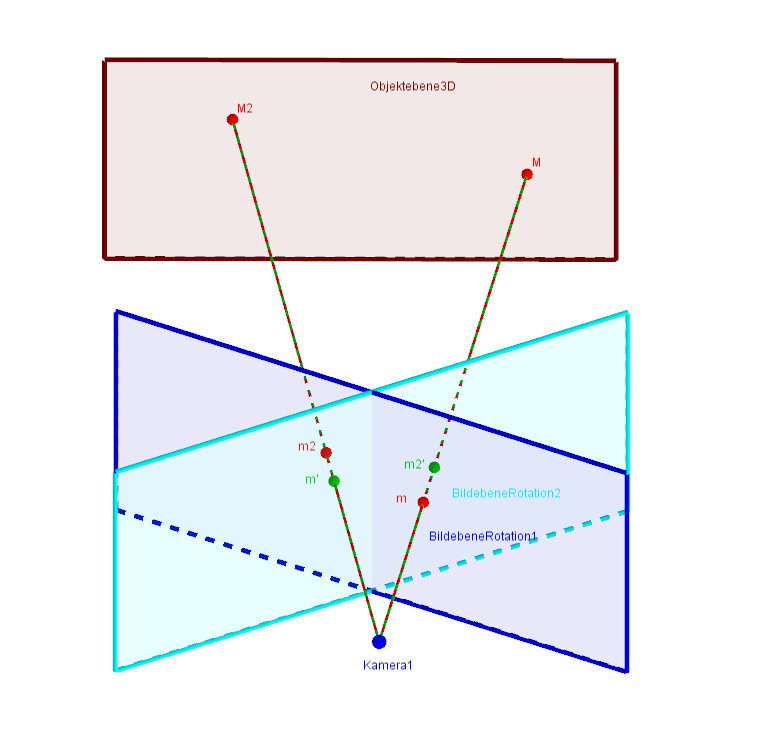
\includegraphics[width=0.8\linewidth]{images/Homographie_rotation_1.png}
	\captionof{figure}{Veranschaulichung von Homographie mit nur einer rotierten Kamera.}
\end{minipage}\\ \\

\begin{minipage}{\linewidth}
	\centering
	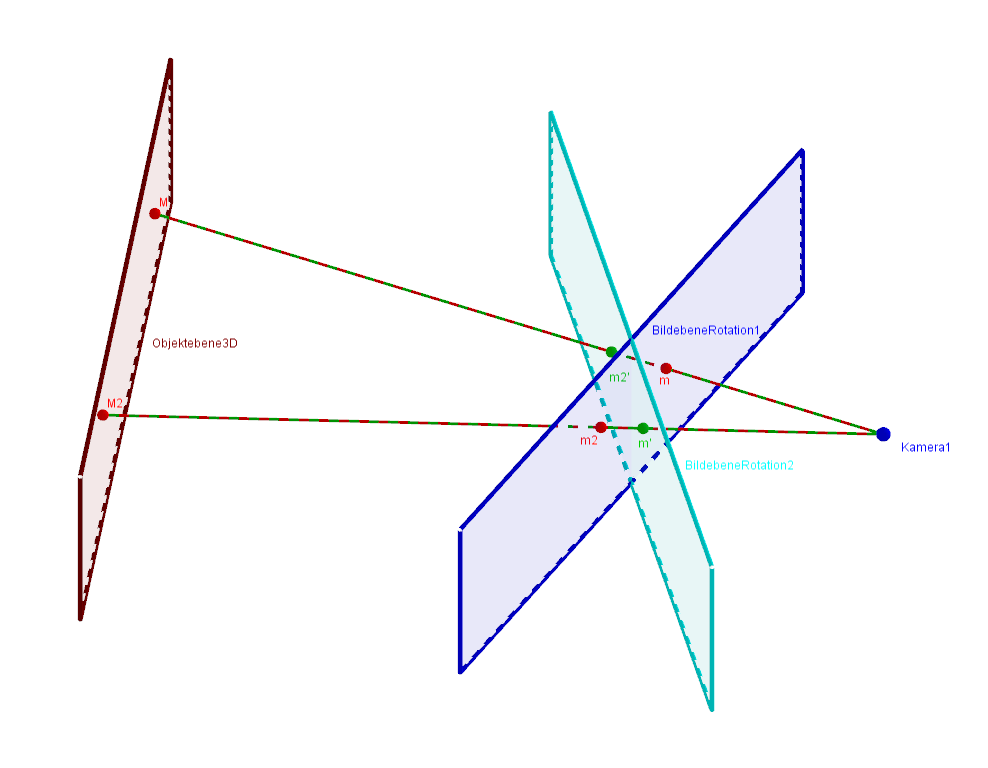
\includegraphics[width=0.8\linewidth]{images/Homographie_rotation_2.png}
	\captionof{figure}{Veranschaulichung von Homographie mit nur einer rotierten Kamera.}
\end{minipage}\\ \\

Die Umrechnung des Objektpunktes $M_\delta$ zu den abgebildeten Punkte $m_\beta$ und $m'_\beta$ mit Basis zu ihren jeweiligen Bildebenenkoordinatensystemem $(o, \beta)$ und $(o',\beta')$ funktioniert wie bereits von den Transformationen in den vorherigen Kapitel bekannt. Hier wird der Vorgang nochmal symbolisch in den Gleichungen 3.7 und 3.8 aufgeführt. Die Projektionsmatrizen, welche die Rotationen und Abbildungsmatrizen der einzelnen Kameras zusammenfasst wird hier mit $P$ für Kamer eins  und $P'$ für Kamera zwei abgekürzt.\cite{Elements}

\begin{gather}
\gamma \vec{m}_\beta = P \begin{bmatrix}\vec{M}_\delta\\1\end{bmatrix} = 
\begin{bmatrix}KR|-KR\vec{C}_\delta\end{bmatrix}\cdot \begin{bmatrix}\vec{M}\delta\\11\end{bmatrix} = KR(\vec{M}\delta - \vec{C}_\delta)\\
\gamma' \vec{m'_{\beta'}} = P' \begin{bmatrix}\vec{M'}_\delta\\1\end{bmatrix} = 
\begin{bmatrix}K'R'|-K'R'\vec{C}_\delta\end{bmatrix}\cdot \begin{bmatrix}\vec{M}\delta\\11\end{bmatrix} = K'R'(\vec{M}\delta - \vec{C}_\delta)
\end{gather}
%Danach wird dann die Beziehung von Punkten im Raum aufgezeigt, welche sich nicht auf einer Ebene befinden. Die Relationen dieser Punkte zueinander lassen sich mit der so genannten Epipolargeometrie beschreiben. Mehr dazu ab Kapitel (link zu Kapitel 3.3
Der Vektor $(\vec{M}\delta - \vec{C}_\delta)$, beschreibt die Verbindung zwischen dem Objektpunkt $M_\delta$ der Objektebene im Raum und dem Projektionszentrum $C_\delta$ im Raum. Die Gleichung sind bereits aus Kapitel \nameref{sec:basisTransformation},Gleichungen 2.73 oder 2.74, bekannt. Es handelt sich hier lediglich wieder um eine Transformation von einem Punkt in 3D Weltkoordinaten über einen Punkt eines 3D- Kamerakoordinatensystems, in 2D-Bildkoordinaten. Jetzt soll aber gezeigt werden, dass die Bildpunkte nur mit einer Homographiematrix, ohne Kenntniss der Kameraparameter ineinander überführt werden können und das alles nur mit den beiden Bildkoordinaten $m_\beta$ und $m'_{\beta}$. Dazu wird im folgenden erst einmal aufgeführt, wie man aus Gleichung 3.7 und 3.8 die Homographiematrix $H$ gewinnen kann. Was bei den zwei Gleichungen auffällt ist, dass die rechte Seite der Gleichungen, die Ergebnisse nur in ihren Kameraparametern $KR$ und $RK$ unterscheiden, während der Vektor $(\vec{M}-\vec{C}_\delta)$, der selbe ist. Das liegt daran, dass zuvor festgelegt wurde, dass die Kameras identische Projektionszentren besitzen. Also gilt $\vec{C_{1\delta}} = \vec{C_{2\delta}} = \vec{C_{\delta}}$. Mit Hilfe dieser Bedinung können wir die Gleichungen gleichsetzten und für $H$ das folgende Ergebnis herleiten. 


\begin{gather}
	\gamma RK^{-1}\vec{m_\beta} = \vec{M}_\delta - \vec{C}_\delta\\
	\gamma' R'K'^{-1}\vec{m'_{\beta'}} = \vec{M}_\delta - \vec{C}_\delta\\
	\leadsto \gamma' R'K'^{-1}\vec{m'_{\beta'}}=\gamma RK^{-1}\vec{m_\beta}\\
	\frac{\gamma'}{\gamma}\vec{m'_{\beta'}} = K'R'R^TK^{-1}\vec{m}_\beta\\
	\lambda \vec{m'}_{\beta'} = H\vec{m}_\beta
\end{gather}

Es Resultiert also dass wenn $\lambda = \frac{\gamma'}{\gamma}$, dann gilt dass $H = K'R'R^TK^{-1}$ gleicht. Gilt nun noch der Fall, dass $K = K'$ ist, dann reduziert sich $H$ zu $K^{-1}HK = R'R$, welches einer schlichten Rotation gleicht.\cite{Elements}




\section{Homographien bei Drehungen um ein Projektionszentrum}

%Homographie zwischen der Abbildungen eines Quadrates einer definierten Ausgangskamera und einer um ihr Projektionszentrum rotierten Kamera
In diesem Beispiel werden die abgebildeten Punkte eines Quadrats einer Kamera $(C_\beta)$ mit $\beta= [\vec{b_1},\vec{b_2},\vec{b_3},C]$ in die einer anderen Kamera $(C',\beta')$ mit $\beta'= [\vec{b'_1},\vec{b'_2},\vec{b'_3},C']$  mit Hilfe einer selbst aufgestellten Homographiematrix überführt. Hierzu wird zunächst eine Szene mit den Eckpunkten des Quadrates $A_\delta, B_\delta, C_\delta, D_\delta$ und dessen Mittelpunkt mit $E_\delta$ und zwei Kameras $C_{\delta}$ und $C'_{\delta}$ definiert. Für Die Projektionszentren der Kameras gilt in hier, dass $C'_{\delta} = C_\delta$. Die Eckpunkte so wie die Kameras werden in Weltkoordinaten mit den Basen $(O,\delta)$ mit $\delta = [\vec{d_1},\vec{d_1},\vec{d_1},O]$ angegeben. Mit Hilfe der gelernten Transformationsmethoden, werden die Eckpunkte in ihre jeweiligen 2D-Bildebenenkooridnaten $(I,\tau)$ und $(I',\tau')$ umgerechnet. Nachdem die Szene vollständig definiert und die auf den Kameras abgebildeten Punkte berechnet sind, werden zwei Methoden gezeigt, mit welchem die Homographiematrix ermittelt werden kann. Da es sich in diesem Beispiel um ein selbst aufgestelltes Minimalbeispiel handelt, kommt es zu keinem überbestimmten Fall bei der der Berechnung der Homographiematrize. Da in Realbeispielen, jedoch immer damit gerechnet werden muss, dass es zu einem überbestimmten Fall kommt, wird das Verfahren, welches diesen Fall abdeckt ebenfalls aufgezeigt. Der Szenenaufbau des Minimalbeispiels soll folgendermaßen aussehen. Die Kamerakoordinatensysteme unterscheiden sich vom Weltkoordinatensystem durch eine Drehung um 180° um die \ensuremath{\vec{d}_1}-Achse. Der Ursprung beider Kamerakoordinatensysteme entspricht dem Projektionszentrum $C$. Des Weiteren ist Kamera zwei noch um $45^\circ$ um die $\vec{b_2}$ zu Kamera eins eingedreht. Es werden zwei Bilder der selben Szene mit diesen Kameras aufgenommen. Die Behauptung ist, dass sich die beiden entstandenen Bilder mit Einer Homographie ineinander überführen lassen. In Abbildung \ref{fig:Koordinatensysteme2} ist der Aufbau nochmal grafisch veranschaulicht.

\begin{gather}
H=
\begin{bmatrix}
h_{11}&h_{12}&h_{13}\\
h_{21}&h_{22}&h_{23}\\
h_{31}&h_{32}&h_{33}
\end{bmatrix}
\end{gather}\\


\begin{minipage}{\linewidth}
	\centering
	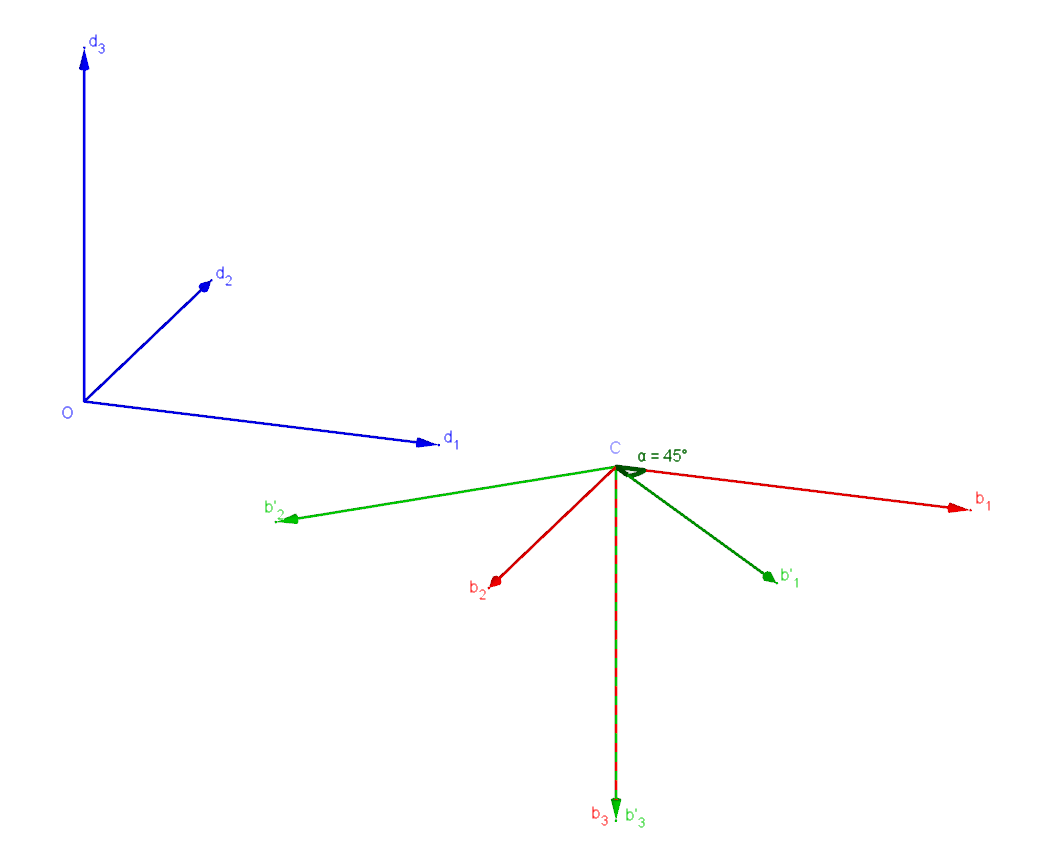
\includegraphics[width=1.\linewidth]{images/GrafikHomographieSameC.png}
	\captionof{figure}{Weltkoordinatensystem $(O,\delta)$ mit $\delta = [\vec{d_1},\vec{d_1},\vec{d_1},O]$ und Kamerakoordinatensysteme $\beta= [\vec{b_1},\vec{b_2},\vec{b_3},C]$ und $(C',\beta')$ mit $\beta'= [\vec{b'_1},\vec{b'_2},\vec{b'_3},C']$ .}
	\label{fig:Koordinatensysteme2}
\end{minipage}\\ \\

Als nächstes werden die intrinsischen Kameraparameter $K$ und $K'$ für beide Kameras festgelegt. Für das Beispiel

\begin{gather}
K=K'
= 
\begin{pmatrix}
\zeta&0&0&0\\
0&\zeta&0&0\\
0&0&\zeta&0\\
0&0&1&0
\end{pmatrix}\\
\leadsto
\begin{pmatrix}
X\\Y\\Z
\end{pmatrix} = 
K
\begin{pmatrix}
X\\Y\\Z\\1
\end{pmatrix}
=
\begin{pmatrix}
\zeta X\\\zeta Y\\\zeta Z\\Z
\end{pmatrix}
=
\begin{pmatrix}
\frac{\zeta}{Z} X\\\frac{\zeta}{Z} Y\\\zeta\\1
\end{pmatrix}
\end{gather}\\

Für das Beispiel gilt die Bedingung, dass $\zeta \neq 0$ sein soll. Des Weiteren soll gelten, dass  \ensuremath{\vec{b}_1} gleich der Lotgeraden vom Objektpunkt zum Projektionszentrum entsptricht und somit folgt, dass \ensuremath{\vec{b}_1} in Sensorebene liegt und \ensuremath{\vec{b}_2 = \vec{b}_3 \times \vec{b}_1} ist. Der Quader besteht aus den Punkten $A_\delta,B_\delta,C_\delta, D_\delta$ und $E\delta$ in homogenen Weltkoordinaten. Die Punkte in Weltkoordinaten bekommen die Koordinatenwerte zugewiesen. 

\begin{gather}
A_\delta=\begin{pmatrix}
0\\0\\2\\1
\end{pmatrix}, 
B_\delta=
\begin{pmatrix}
1\\0\\2\\1
\end{pmatrix},
C_\delta=
\begin{pmatrix}
1\\1\\2\\1
\end{pmatrix},
D_\delta=
\begin{pmatrix}
0\\1\\2\\1
\end{pmatrix},
E_\delta=
\begin{pmatrix}
\frac{1}{2}\\\frac{1}{2}\\2\\1
\end{pmatrix}
\end{gather}\\

Für die Transformation der Weltkoordinatentupel in die Bildebenen $I$ und $I'$ werden die Projektionsmatrizen $P=[KR|-KRC_\delta]$ und $P'=[K'R'|-K'R'C_\delta]$ aufgestellt werden. \ensuremath{R} soll eine Drehung der Punkte um 180° um die \ensuremath{\vec{d}_1}-Achse druchführen. \ensuremath{R'} muss zusätzlich im Anschluss noch eine Drehung, um \ensuremath{45^\circ} um die neue $\vec{b'_3}$-Achse von Kamera zwei, an die vorherige Drehung anhängen. Die so erhaltenen Matrizen \ensuremath{R} und \ensuremath{R'} können nun dazu verwendet werden, die Objektpunkte bezüglich des Weltkoordinatensystems $(O,\delta)$ in Punkte bezüglich der jeweiligen Kamerakoordinatensysteme $(C,\beta)$ und $(C',\beta')$ zu transformieren.


\begin{gather}
	\begin{bmatrix}
		\cos(180)&-\sin(180)&0&0\\
		\sin(180)&\cos(180)&0&0\\
		0&0&1&0\\
		0&0&0&1
	\end{bmatrix}
	\begin{pmatrix}
		\vec{d}_1,\vec{d}_2,\vec{d}_3,O
	\end{pmatrix}
	=
	\begin{bmatrix}
		-1&0&0&0\\
		0&-1&0&0\\
		0&0&1&0\\
		0&0&0&1
	\end{bmatrix} 
	\begin{pmatrix}
		\vec{d}_1,\vec{d}_2,\vec{d}_3,O
	\end{pmatrix}\\
	\begin{bmatrix}
		-1&0&0&0\\
		0&-1&0&0\\
		0&0&1&0\\
		0&0&0&1
	\end{bmatrix}^T =\begin{bmatrix}
	-1&0&0&0\\
	0&-1&0&0\\
	0&0&1&0\\
	0&0&0&1
	\end{bmatrix}= R
\end{gather}\\

Im nächsten Schritt wird Kamera zwei noch um \ensuremath{45^\circ} um ihre $\vec{b'_3}$-Achse gedreht. Diese Transformation wird mit der vorherigen Transformation multipliziert und es entsteht $P'$ für Kamera zwei.

\begin{gather}
	\cos(45)=\sin(45)=\frac{1}{\sqrt{2}} = a\\
	\begin{bmatrix}
		a&0&a&0\\
		0&1&0&0\\
		-a&0&a&0\\
		0&0&0&1
	\end{bmatrix}
	\begin{bmatrix}
		-1&0&0&0\\
		0&-1&0&0\\
		0&0&1&0\\
		0&0&0&1
	\end{bmatrix}
	=\begin{bmatrix}
		-a&0&a&0\\
		0&-1&0&0\\
		a&0&a&0\\
		0&0&0&1
	\end{bmatrix}
	\begin{pmatrix}
		\vec{d}_1,\vec{d}_2,\vec{d}_3,O
	\end{pmatrix}\\
	=\begin{bmatrix}
	-a&0&a&0\\
	0&-1&0&0\\
	a&0&a&0\\
	0&0&0&1
	\end{bmatrix}^T
	=
	\begin{bmatrix}
		-a&0&a&0\\
		0&-1&0&0\\
		a&0&a&0\\
		0&0&0&1
	\end{bmatrix}
	= R'
\end{gather}\\

Handelt es sich bei den Kamerakoordinatensystemen nicht um karteische Koordinatensysteme, so muss von den Rotationsmatrizen jeweils die Inverse genommen werden, um \ensuremath{R} und \ensuremath{R'} zu erhalten. Die Inversen Rotationsmatrizen werden in den folgenden Gleichungen nicht mit $R^{-1}$, sondern $R$ bezeichnet. So entsprechen sie auch den Notationen der Literatur\cite{Elements,HZ}. Sind die Matrizen \ensuremath{R} und \ensuremath{R'} ermittelt, können nun die Punkte des Quadrats im Raum in Punkte der jeweiligen Kameras umgerechnet werden. Für Punkte spezifisch Kamera eins ergeben sich die in den Gleichungen 3.23 bis 3.27 aufgezeigten Werte.


\begin{gather}
	\begin{pmatrix}
		A_\beta\\1
	\end{pmatrix}
	=
	\begin{bmatrix}
		-1&0&0&0\\
		0&-1&0&0\\
		0&0&1&0\\
		0&0&0&1
	\end{bmatrix}
	\begin{pmatrix}
		0\\0\\2\\1
	\end{pmatrix}
	=
	\begin{pmatrix}
		0\\0\\2\\1
	\end{pmatrix}\\
	\begin{pmatrix}
		B_\beta\\1
	\end{pmatrix}
	=
	\begin{bmatrix}
		-1&0&0&0\\
		0&-1&0&0\\
		0&0&1&0\\
		0&0&0&1
	\end{bmatrix}
	\begin{pmatrix}
		1\\0\\2\\1
	\end{pmatrix}
	=
	\begin{pmatrix}
		-1\\0\\2\\1
	\end{pmatrix}\\
	\begin{pmatrix}
		C_\beta\\1
	\end{pmatrix}
	=
	\begin{bmatrix}
		-1&0&0&0\\
		0&-1&0&0\\
		0&0&1&0\\
		0&0&0&1
	\end{bmatrix}
	\begin{pmatrix}
		1\\1\\2\\1
	\end{pmatrix}
	=
	\begin{pmatrix}
		-1\\-1\\2\\1
	\end{pmatrix}\\
	\begin{pmatrix}
		D_\beta\\1
	\end{pmatrix}
	=
	\begin{bmatrix}
		-1&0&0&0\\
		0&-1&0&0\\
		0&0&1&0\\
		0&0&0&1
	\end{bmatrix}
	\begin{pmatrix}
		0\\1\\2\\1
	\end{pmatrix}
	=
	\begin{pmatrix}
		0\\-1\\2\\1
	\end{pmatrix}\\
	\begin{pmatrix}
	E_\beta\\1
\end{pmatrix}
=
\begin{bmatrix}
	-1&0&0&0\\
	0&-1&0&0\\
	0&0&1&0\\
	0&0&0&1
\end{bmatrix}
\begin{pmatrix}
	\frac{1}{2}\\\frac{1}{2}\\2\\1
\end{pmatrix}
=
\begin{pmatrix}
	-\frac{1}{2}\\-\frac{1}{2}\\2\\1
\end{pmatrix}
\end{gather}

Für Punkte spezifisch Kamera zwei ergeben sich die Punkte aus den Gleichungen 3.28 bis 3.32.

\begin{gather}
	\begin{pmatrix}
		A'_{\beta'}\\1
	\end{pmatrix}
	=
	\begin{bmatrix}
		-a&0&a&0\\
		0&-1&0&0\\
		a&0&a&0\\
		0&0&0&1
	\end{bmatrix}
	\begin{pmatrix}
		0\\0\\2\\1
	\end{pmatrix}
	=
	\begin{pmatrix}
		2a\\0\\2a\\1
	\end{pmatrix}\\
	\begin{pmatrix}
		B'_{\beta'}\\1
	\end{pmatrix}
	=
	\begin{bmatrix}
		-a&0&a&0\\
		0&-1&0&0\\
		a&0&a&0\\
		0&0&0&1
	\end{bmatrix}
	\begin{pmatrix}
		1\\0\\2\\1
	\end{pmatrix}
	=
	\begin{pmatrix}
		a\\0\\3a\\1
	\end{pmatrix}\\
	\begin{pmatrix}
		C'_{\beta'}\\1
	\end{pmatrix}
	=
	\begin{bmatrix}
		-a&0&a&0\\
		0&-1&0&0\\
		a&0&a&0\\
		0&0&0&1
	\end{bmatrix}
	\begin{pmatrix}
		1\\1\\2\\1
	\end{pmatrix}
	=
	\begin{pmatrix}
		a\\-1\\3a\\1
	\end{pmatrix}\\
	\begin{pmatrix}
		D'_{\beta'}\\1
	\end{pmatrix}
	=
	\begin{bmatrix}
		-a&0&a&0\\
		0&-1&0&0\\
		a&0&a&0\\
		0&0&0&1
	\end{bmatrix}
	\begin{pmatrix}
		0\\1\\2\\1
	\end{pmatrix}
	=
	\begin{pmatrix}
		2a\\-1\\2a\\1
	\end{pmatrix}\\
	\begin{pmatrix}
	E'_{\beta'}\\1
\end{pmatrix}
=
\begin{bmatrix}
	-a&0&a&0\\
	0&-1&0&0\\
	a&0&a&0\\
	0&0&0&1
\end{bmatrix}
\begin{pmatrix}
	\frac{1}{2}\\\frac{1}{2}\\2\\1
\end{pmatrix}
=
\begin{pmatrix}
	\frac{3}{2}a\\-\frac{1}{2}\\\frac{5}{2}a\\1
\end{pmatrix}
\end{gather}\\

Die entstandenen Punkte sind nun entsprechend der Kamerakoordinatensysteme definiert. Jetzt müssen noch die jeweiligen Kameramatrizen $K$ und $K'$ mit diesen verrechnet werden, um so die 2D-Bildebenenpunkte der entsprechenden Kameras zu erhalten. $\zeta$ bekommt in diesem Beispiel den Wert -1, das bedeutet laut der Definition der Kamerakoordinatensysteme, dass der Sensor sich hinter dem Projektionszentrum befindet. Das entstehende Bild ist somit um \ensuremath{180^\circ} gedreht auf dem Sensor abgebildet.

\begin{gather}
K =	K'=
	\begin{pmatrix}
		\zeta&0&0&0\\
		0&\zeta&0&0\\
		0&0&\zeta&0\\
		0&0&1&0
	\end{pmatrix}=
	\begin{pmatrix}
		-1&0&0&0\\
		0&-1&0&0\\
		0&0&-1&0\\
		0&0&1&0
	\end{pmatrix}
\end{gather}

 Man kann natürlich wie bereits gewohnt die Rotationsmatrizen und die Kameramatrizen bereits im Vorhinein miteinander multiplizieren und dann auf einen 3D-Weltpunkt anwenden. Auf diese Weise bekommt man die fertigen Projektionsmatrizen  $P=[KR|-KRC_\delta]$ und $P'=[K'R'|-K'R'C_\delta]$. In diesem Beispiel werden sie nochmal getrennt voneinander auf die Punkte angewandt. Die fünf Punkte werden jeweils in einer Matrix zusammengeschrieben und mit $K$ beziehungsweise $K'$ verrechnet. 

\begin{gather}
K \cdot 
	\begin{pmatrix}
0&-1&-1&0&-\frac{1}{2}\\
0&0&-1&-1&-\frac{1}{2}\\
2&2&2&2&2\\
1&1&1&1&1
\end{pmatrix}=
	\begin{pmatrix}
		-1&0&0&0\\
		0&-1&0&0\\
		0&0&-1&0\\
		0&0&1&0
	\end{pmatrix}
	\begin{pmatrix}
		0&-1&-1&0&-\frac{1}{2}\\
		0&0&-1&-1&-\frac{1}{2}\\
		2&2&2&2&2\\
		1&1&1&1&1
	\end{pmatrix}\\=
	\begin{pmatrix}
		0&1&1&0&-\frac{1}{2}\\
		0&0&1&1&-\frac{1}{2}\\
		-2&-2&-2&-2&-2\\
		2&2&2&2&2
	\end{pmatrix}\\
	\simeq
	\begin{pmatrix}
		0&\frac{1}{2}&\frac{1}{2}&0&\frac{1}{4}\\
		0&0&\frac{1}{2}&\frac{1}{2}&\frac{1}{4}\\
		-1&-1&-1&-1&-1\\
		1&1&1&1&1
	\end{pmatrix}	
	\simeq
	\begin{pmatrix}
	0&\frac{1}{2}&\frac{1}{2}&0&\frac{1}{4}\\
	0&0&\frac{1}{2}&\frac{1}{2}&\frac{1}{4}\\
	1&1&1&1&1
	\end{pmatrix}\\
K' \cdot 	\begin{pmatrix}
2a&a&a&2a&\frac{3}{2}a\\
0&0&-1&-1&-\frac{1}{2}\\
2a&3a&3a&2a&\frac{5}{2}a\\
1&1&1&1&1
\end{pmatrix}=
	\begin{pmatrix}
		-1&0&0&0\\
		0&-1&0&0\\
		0&0&-1&0\\
		0&0&1&0
	\end{pmatrix}
	\begin{pmatrix}
		2a&a&a&2a&\frac{3}{2}a\\
		0&0&-1&-1&-\frac{1}{2}\\
		2a&3a&3a&2a&\frac{5}{2}a\\
		1&1&1&1&1
	\end{pmatrix}\\=
	\begin{pmatrix}
		-2a&-a&-a&-2a&-\frac{3}{2}a\\
		0&0&1&1&\frac{1}{2}\\
		-2a&-3a&-3a&-2a&-\frac{5}{2}a\\
		2a&3a&3a&2a&\frac{5}{2}a
	\end{pmatrix}\\
	\simeq
	\begin{pmatrix}
		-1&-\frac{1}{3}&-\frac{1}{3}&-1&\frac{3}{5}\\
		0&0&\frac{1}{3a}&\frac{1}{2a}&\frac{1}{5}a\\
		-1&-1&-1&-1&-1\\
		1&1&1&1&1
	\end{pmatrix}
		\simeq
	\begin{pmatrix}
	-1&-\frac{1}{3}&-\frac{1}{3}&-1&\frac{3}{5}\\
	0&0&\frac{1}{3a}&\frac{1}{2a}&\frac{1}{5a}\\
	1&1&1&1&1
	\end{pmatrix}
\end{gather}\\

Die Entstandenen Punkte beider Kameras ergeben die in Abblidung \ref{ErgebniseHomographie1} veranschaulichten Abblildungen, des Quadrats mit seinem Mittelpunkt, auf den jeweiligen Kamerabildebenen. Die aus den Objektpunkten $M_\delta$ entstandenen 2-D-Bildebenenkoordinaten $m_\tau$ und $m'_{\tau'}$ werden in den Koordinatensystemen $(I,\tau)$ mit $(\tau = \vec{b_1},\vec{b_2},\vec{b_4})$ und $(I',\tau')$ mit $(\tau = \vec{b'_1},\vec{b'_2},\vec{b'_4})$ dargestellt.\\

\begin{minipage}{\linewidth}
	\centering
	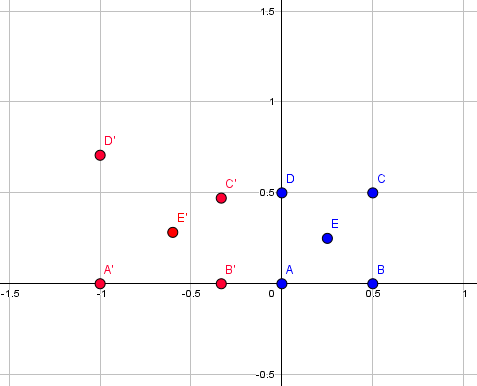
\includegraphics[width=0.8\linewidth]{images/Geogebra.png}
	\captionof{figure}{in blau ist die Abblidung des Quaders von Kamera eins und in rot die Abbildung des selben Quaders in Kamera zwei}
	\label{ErgebniseHomographie1}
\end{minipage}\\ \\

Die fertigen Bildebenenkoordinaten beider Kameras, sollen nun durch eine eigens aufgestellte Homographiematrix $H$ ineinander überführt werden. Um eine Homographiematrix mit 
$H=
\begin{bmatrix}
h_{11}&h_{12}&h_{13}\\
h_{21}&h_{22}&h_{23}\\
h_{31}&h_{32}&h_{33}
\end{bmatrix}
$ zu erhalten werden die Punkte beider Kameras in eine Koeffizientenmatrix eingetragen, welche sich nach dem in den Gleichungen 4.40 bis 3.52 laufenden Schema ergibt. Das Verfahren wird anhand der Bildebenekoordinagen aufgezeigt.

\begin{gather}
H\cdot m_\tau = m'_{\tau}\\
\begin{bmatrix}
h_{11}&h_{12}&h_{13}\\
h_{21}&h_{22}&h_{23}\\
h_{31}&h_{32}&h_{33}
\end{bmatrix}
\cdot
\begin{bmatrix}
\\m_\tau\\\\
\end{bmatrix}
=
\begin{bmatrix}
\\m'_{\tau'}\\\\
\end{bmatrix}\\
\begin{bmatrix}
h_{11}&h_{12}&h_{13}\\
h_{21}&h_{22}&h_{23}\\
h_{31}&h_{32}&h_{33}
\end{bmatrix}
\cdot
\begin{bmatrix}
x\\y\\z
\end{bmatrix}
=
\begin{bmatrix}
x'\\y'\\z'
\end{bmatrix}
\end{gather}

Aus Gleichung 3.42 lassen sich ein Gleichungssystem mit zwölf Bekannten und neun unbekannten aufstellen.  

\begin{gather}
h_{11}x+h_{12}y+h_{13}z= \lambda x'\\
h_{21}x+h_{22}y+h_{23}z= \lambda y'\\
h_{31}x+h_{32}y+h_{33}z= \lambda z'
\end{gather}

Da mit homogenen Koordinaten gearbeitet wird und somit $z$ und $z'$ = 1 sind, ergibt sich für die letzte Zeile $h_{31}x+h_{32}y+h_{33}z= 1$. Dieser Ausdruck kann in den ersten beiden Gleichungen für $\lambda$ eingesetzt werden. Pro Punktepaar $m_\tau$ und $m'_{\tau'}$ ergeben sich somit zwei Gleichungen. 

\begin{gather}
	h_{11}x+h_{12}y+h_{13}z= (h_{31}x+h_{32}y+h_{33}z) \cdot x'\\
		h_{21}x+h_{22}y+h_{23}z= (h_{31}x+h_{32}y+h_{33}z) \cdot y'
\end{gather}

Für den Aufbau der nötigen Koeffizientenmatrix werden beide Ausdrücke noch nach Null aufgelöst, so dass sich die Gleichungen 3.48 und 3.49 aus 3.46 und 3.47 ergeben.

\begin{gather}
	h_{11}x+h_{12}y+h_{13}z -(h_{31}x+h_{32}y+h_{33}z) \cdot x'= 0 \\	h_{21}x+h_{22}y+h_{23}z-(h_{31}x+h_{32}y+h_{33}z) \cdot y'=0
	\end{gather}
\begin{gather}
	\leadsto h_{11}x+h_{12}y+h_{13}z -h_{31}x\cdot x' - h_{32}y \cdot x'-h_{33}z\cdot x'= 0\\
	\leadsto h_{21}x+h_{22}y+h_{23}z-h_{31}x\cdot y -h_{32}y \cdot y -h_{33}z) \cdot y'=0
\end{gather}

Die enstandnen Gleichungen werden jetzt pro Punktepaar $m_\tau$ und $m'_{\tau'}$ in eine Matrix nach folgendem Schema eingetragen.\cite{Elements,HZ,Schwarz,Heipke}

\begin{gather}
	\begin{pmatrix}
	x_1&y_1&1&0&0&0&x_1 x'_1&y_1 x'_1 & 1\cdot x'_1\\
	0&0&0&x_1&y_1&1&x_1 y'_1&y_1 y'_1 & 1\cdot y'_1\\
	&&&&&.&&&\\	
	&&&&&.&&&\\	
	&&&&&.&&&\\	
	x_i&y_i&1&0&0&0&x_i x'_i&y_i x'_i & 1\cdot x'_i\\
	0&0&0&x_i&y_i&1&x_i y'_i&y_i y'_i & 1\cdot y'_i
	\end{pmatrix}
	\cdot
	\begin{pmatrix}
	h1\\h2\\.\\.\\.\\hi
	\end{pmatrix}
	=0
\end{gather}

Wenn ein nicht überbestimmter Fall vorliegt, sprich wenn der Rang der Koeffizientenmatrix genau acht und nicht höher beträgt, kann aus der Koeffizientenmatrix einfach der Nullraum berechnet werden, um so die Einträge für die 3x3-Homographiematrix zu erhalten\cite{HZ,Elements,Schwarz}. Gesucht wird also ein Vector $\vec{x}$, für den gilt das $H \cdot x = 0$. Der gesuchte Vektor $\vec{x}$ entspricht dem Kern der Koeffizientenmatrix und ist ein Spaltenvektor mit 9 Einträgen, welche in die 3x3-Homographiematrix eingetragen werden können\cite{HZ,Schwarz}. Tritt nun der Fall ein, dass es zu einem überbestimmtes System kommt, \textcolor{red}{was Beipielsweise auftritt wenn mehr als neun Punktepaare durch eine Homographie ineinander überführt werden sollen}, so kann nicht mehr die Ermittlung des Nullraums für die Berechnung der Homographiematrix genutzt werden. Für die Lösung überbestimmter Gleichungssysteme bietet sich die Singulärwertzerlegung an\cite{HZ}\cite{Scholz}. Das bedeutet es wird nicht derjenige Vektor $\vec{x}$ gesucht für den gilt $H \cdot x = 0$, sondern es wird derjenige Vektor $\vec{x}$ gesucht, für den \ensuremath{\parallel H \cdot x\parallel} minimal wird\cite{HZ,Schwarz}. Die Singulärwertzerlegung von zum Beispiel der Koeffizientenmatrix ist eine Faktorisierung einer beliebeigen Matrix \ensuremath{A \in \mathbb{R}^{mxn}} der Form \ensuremath{A = U \cdot S \cdot V^T} mit orthogonalen Matrizen \ensuremath{U \in \mathbb{R}^{m \times n}} und \ensuremath{V \in \mathbb{R}^{m \times n}} sowie mit einer Diagonalmatrix. 

\begin{gather}
	S = \begin{pmatrix}
	s_1&&...&&0&0&&...&&0\\
	.&.&&&.&.&&&&.\\
	.&&.&&.&.&&&&.\\
	.&&&.&.&.&&&&.\\
	0&&...&&s_r&0&&...&&0\\	
	0&&...&&0&0&&...&&0\\
	.&&&&.&.&&&&.\\
	.&&&&.&.&&&&.\\	
	.&&&&.&.&&&&.\\	
	0&&...&&0&0&&...&&0\\	
	\end{pmatrix}
\end{gather}

Dabei soll für die Singulärwerte $s_1$ bis $s_r$ gelten, dass \ensuremath{s_1 \geq s_2 \geq ... \geq s_r \ge 0 }\cite{Scholz}. Entsprechend dieser Methode wird eine Singulärwertszerlegung, kurz $SVD$ der entstandenen Koeffizientenmatrix durchgeführt. Wir erhalten 3 Matrizen $U \cdot S\cdot V^T$. Durch die Zerlegung sind die diagonaleinträge von $S$ in einer absteigenden Reihenfolge sortiert. Die Spalte von $V^T$, welche mit dem kleinsten Singulärwert von $S$ korrespondiert, ergibt den Vektor $\vec{x}$, für den \ensuremath{\parallel H \cdot x\parallel} minimal wird. Somit gleichen die neun Einträge der Homographiematrix gleich der letzten Spalte von $V$. Das Ergebnis für $H$ hat dann die folgende Form

\begin{gather}
	H=
	\begin{pmatrix}
	v_{19}&v_{29}&v_{39}\\
	v_{49}&v_{59}&v_{69}\\
	v_{79}&v_{89}&v_{99}
	\end{pmatrix}
\end{gather}

Für das Minimalbeispiel mit reinen Punkten, welches in diesem Kapitel erstellt wurde, würde die Herleitung der Homographiematrix über die Ermittlung des Nullraumes der Koeffizientenmatrix genügen. Für die Matrix $H$ ergibt sich aus den Werten der im Beispiel verwendeten Punkte

\begin{gather}
	\begin{pmatrix}
	1&0&-1\\
	0&\sqrt{2}&0\\
	1&0&1
	\end{pmatrix}
\end{gather}

Nun werden die Punkte aus Kamera eins s mit Hilfe von $H$ in die Punkte von Kamera zwei überführt und umgekehrt werden die Punkte aus Kamera zwei mit der Inversen $H^{-1}$ in die Punkte von Kamera eins überführt. 

\begin{gather}
x'=H \cdot x \leadsto 
	\begin{pmatrix}
	-1&-\frac{1}{3}&-\frac{1}{3}&-1\\
	0&0&\frac{1}{3a}&\frac{1}{2a}\\
	1&1&1&1
\end{pmatrix}= 	\begin{pmatrix}
1&0&-1\\
0&\sqrt{2}&0\\
1&0&1
\end{pmatrix}
\cdot
\begin{pmatrix}
0&\frac{1}{2}&\frac{1}{2}&0\\
0&0&\frac{1}{2}&\frac{1}{2}\\
1&1&1&1
\end{pmatrix}\\
x=H^{-1} \cdot x' \leadsto 
\begin{pmatrix}
0&\frac{1}{2}&\frac{1}{2}&0\\
0&0&\frac{1}{2}&\frac{1}{2}\\
1&1&1&1
\end{pmatrix}
= 	\begin{pmatrix}
\frac{1}{2}&0&\frac{1}{2}\\
0&\frac{1}{\sqrt{2}}&0\\
\frac{1}{2}&0&\frac{1}{2}
\end{pmatrix}
\cdot
\begin{pmatrix}
-1&-\frac{1}{3}&-\frac{1}{3}&-1\\
0&0&\frac{1}{3a}&\frac{1}{2a}\\
1&1&1&1
\end{pmatrix}
\end{gather}

\section{Abbildungsunterschiede bei verschobenen Rotationsachsen}

%Abbildungsunterschiede von Rotationen um ein Projektionszentrum und Rotation um einen beliebigen Drehpunkt von Punkten in der Ebene

Bis jetzt wurden die Kameras jeweils nur um ihr Projektionszentrum gedreht, die Frage die jetzt noch im folgenden beantwortet werden soll ist, ob es ebenfalls möglich ist eine Homographiematrix für korrespondierende Punktepaare in einer Ebene aufzustellen, wenn eine Kamera um einen spezifischen Drehpunkt außerhalb der Kamera gedreht wurde. In diesem Fall wären die beiden Projektionszentren $(C,\beta)$ und $(C',\beta')$ der Kameras nicht mehr identisch. Um zu veranschaulichen, was genau sich bei einer Drehung um ein Drehpunkt und der Drehung um das Projektionszentrum ändert, wurde eine Simulation geschrieben, welche die Abbildungsunterschiede beider Drehungen aufzeigt. Des Weiteren soll geklärt werden, ob Punkte die bei der Drehung um das Projektionszentrum verdeckt bleiben auch bei einer Drehung um einen außerhalb der Kamera platzierten Drehpunkt verdeckt bleiben. In der Simulation ist der rote Punkte in der Mitte des Quadrats der Drehpunkt, wie in Abbildung \ref{fig:SimulationAnfang} dargestellt ist. 

\begin{minipage}{\linewidth}
	\centering
	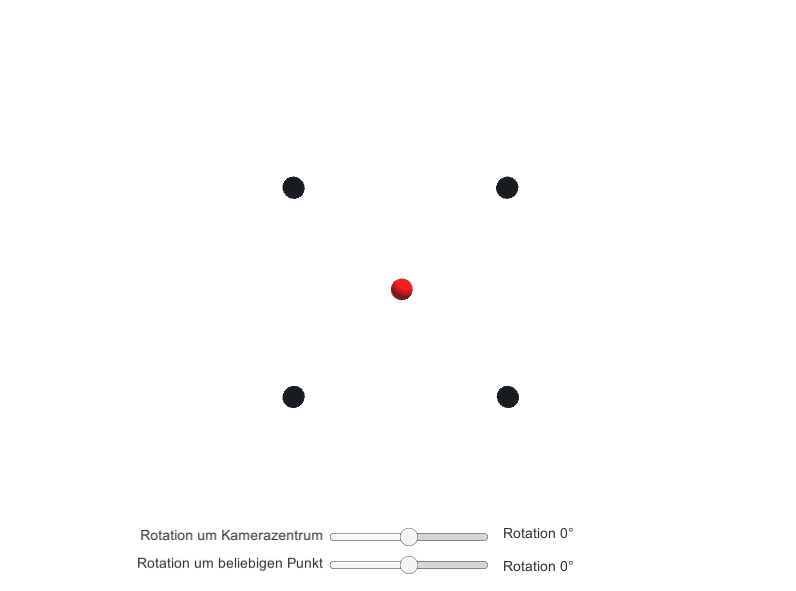
\includegraphics[width=.8\linewidth]{images/Ausgangslage.png}
	\captionof{figure}{Objekt im Raum}
	\label{fig:SimulationAnfang}
\end{minipage}\\


Für die Simulation der Drehung wurden zwei Schieberegler implementiert mit dem sich die Kamera einmal um das Projektionszentrum, und einmal um den Drehpunkt, welcher der rote Mittelpunkt ist, drehen lässt.


\begin{minipage}{\linewidth}
	\centering
	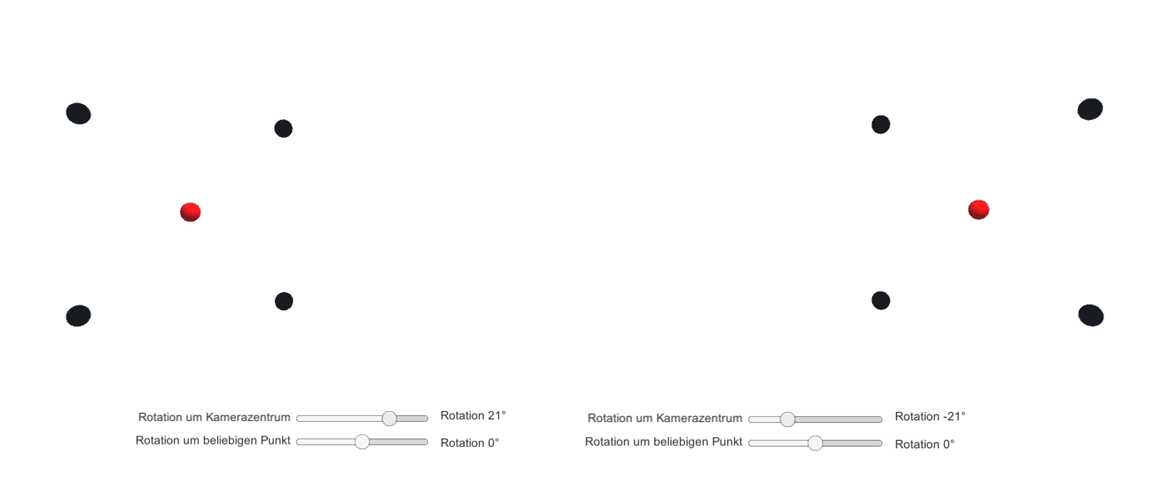
\includegraphics[width=1.\linewidth]{images/DrehungPZ.png}
	\captionof{figure}{Drehung um das Projektionszentrum}
	\label{fig:DrehungProjektionszentrum}
\end{minipage}\\ \\

Abbildung \ref{fig:DrehungProjektionszentrum} zeigt jeweils die entstehenden Bilder, wenn die Kamera um \ensuremath{20^\circ} beziehungsweise \ensuremath{-20^\circ} um das Projektionszentrum gedreht wurde.

\begin{minipage}{\linewidth}
	\centering
	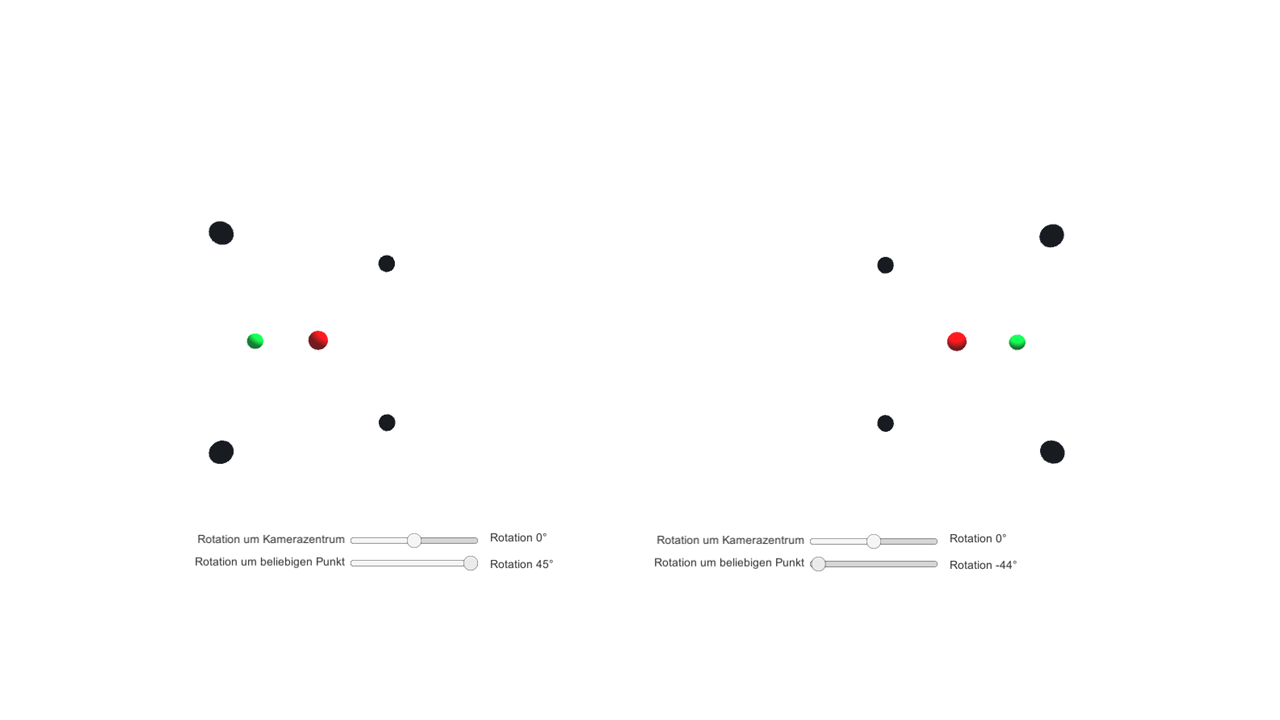
\includegraphics[width=1.\linewidth]{images/DrehungDZ.png}
	\captionof{figure}{Drehung um einen Drehpunkt. In diesem Beispiel wurde der rote Punkt als Drehpunkt verwendet}
	\label{fig:DrehungDrehpunkt}
\end{minipage}\\ 

Abbildung \ref{fig:DrehungDrehpunkt} zeigt die entstehenden Bilder, wenn die Kamera um \ensuremath{45^\circ} beziehungsweise \ensuremath{-45^\circ} um den Drehpunkt gedreht wurde. Wie sich zeigt ist hier ein weiterer grüner Punkt zu sehen welcher zu Testzwecken hinter dem roten Punkt platziert wurde sichtbar. Punkte die bei einer Drehung um das Projektionszentrum verdeckt bleiben, werden also bei einer Drehung um einen externen Drehpukt sichtbar. Die Abbildungen \ref{fig:Strahlengang1} und \ref{fig:Strahlengang2} veranschaulichen was geometrisch bei beiden Fällen passiert.\\

\begin{minipage}{\linewidth}
	\centering
	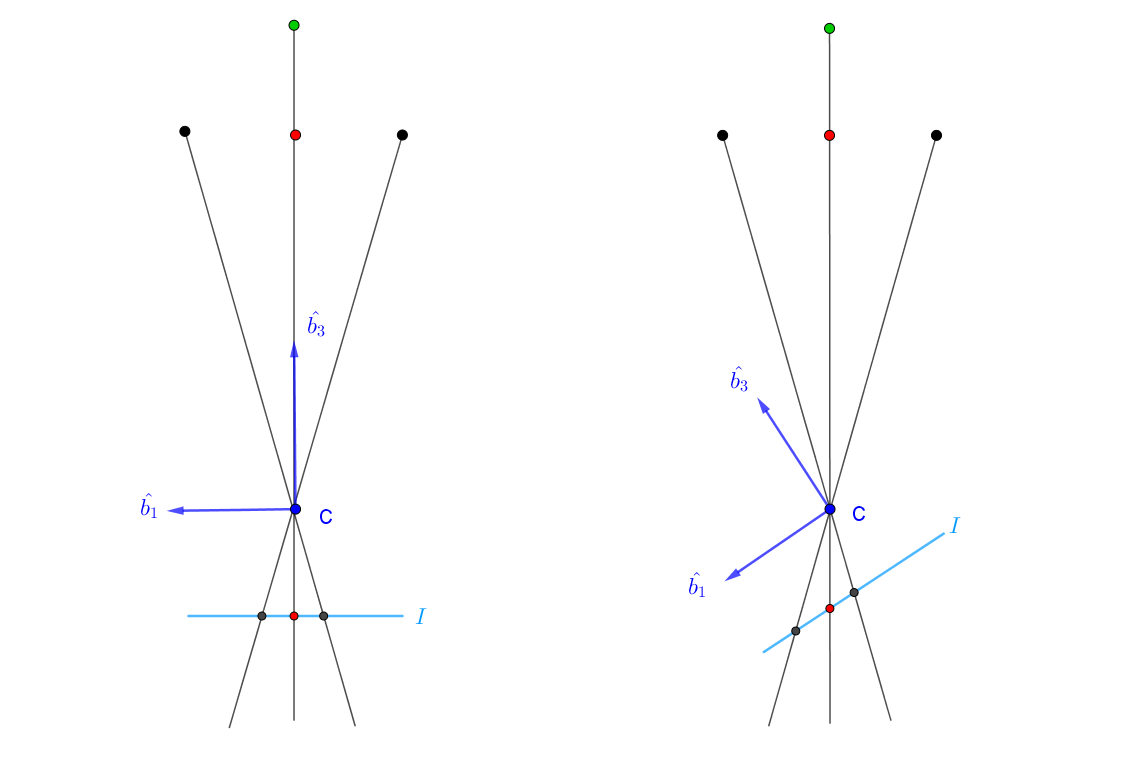
\includegraphics[width=.8\linewidth]{images/GrafikDrehungProjektionszentrum.png}
	\captionof{figure}{Strahlengang durch das Projektionszentrum. Auf der Grafik ist erkennbar, dass der grüne Punkt auch nach der Drehung der Kamera um das Projektionszentrum vom roten Pukt verdeckt bleibt}
	\label{fig:Strahlengang1}
\end{minipage}\\ \\

\begin{minipage}{\linewidth}
	\centering
	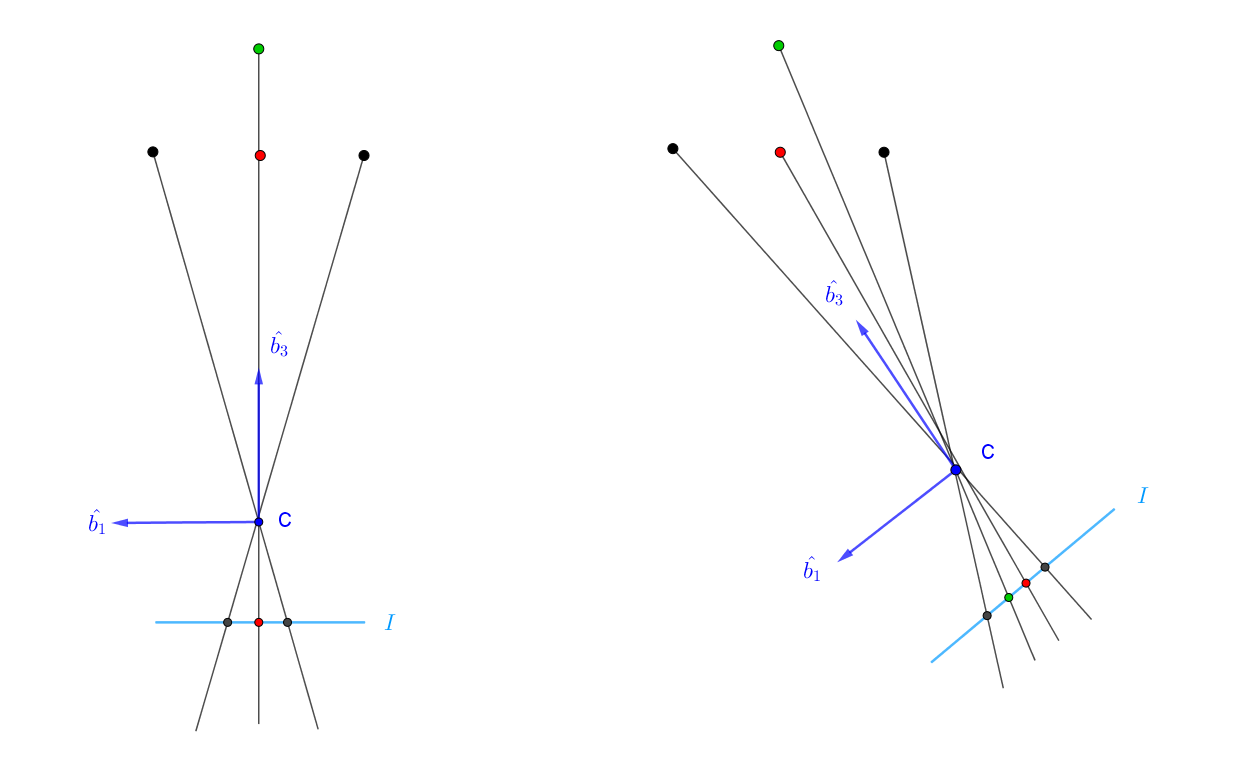
\includegraphics[width=.8\linewidth]{images/GrafikDrehungUmDrehpunkt.png}
	\captionof{figure}{Strahlengang durch das Projektionszentrum. Auf der Grafik ist erkennbar, dass der grüne Punkt nach der Drehung der Kamera um einen Drehpunkt, welcher in diesem Fall der rote Punkt darstellt, sichtbar wird.}
	\label{fig:Strahlengang2}
\end{minipage}\\ \\

Die entstehenden Abbildungen sind also voneinander verschieden, jedoch liegen die fünf Punkte des Quadrates und dessen Mittelpunkt bei beiden Fällen immer noch in einer Ebene. Die Behauptung die also nun noch zu beweisen gilt ist, dass sich für die jeweiligen Abbildungen beider Drehungen jeweils eine Homographiematrix $H$ aufstellen lässt, welche die Bilder der jewiligen Kameras ineinander überführen lässt. Im folgenden wird aufgeführt, wie sich die Homographiematrix im Falle einer Drehung um einen Drehpunkt geometrisch Herleiten lässt. Danach wird wieder ein Beispiel zu diesem Fall aufgezeigt.  Zunächst werden wieder die benötigten Koordinatensysteme definiert. Ein Weltkoordinatensystem $(0,\delta)$ mit $\delta = [\vec{d}_1,\vec{d}_2,\vec{d}_3,O]$, ein Kamerakoordinatensystem von Kamera eins $(C,\beta)$ mit $\beta = [\vec{b}_1,\vec{b}_2,\vec{b}_3,C]$ und ein Kamerakoordinatensystem für Kamera zwei $(C',\beta')$ mit $\beta' = [\vec{b'}_1,\vec{b'}_2,\vec{b'}_3,C']$. Für die Bildebenen $I$ und $I'$ der beiden Kameras gelten die Koordinatensysteme $(I,\vec{\tau})$ und $(I',\vec{\tau}')$ mit $\vec{\tau} = [\vec{d}_1,\vec{d}_2,\vec{d}_4]$ und $\tau' = [\vec{d}_1,\vec{d}_2,\vec{d'}_4]$ mit $d_4 = \vec{CO}$ und $d'_4 = \vec{CO'}$. Der Punkt in der Objektebene, welcher in die jeweiligen Bildebenen projiziert werden soll, wird mit $\vec{M}_\delta = [x\; y\; z\; 1]^T$ bezeichnet. $M$ wird auf die jeweiligen Bildebenen der Kameras projiziert und zu den 2D-Bildebenenkoordinaten $m = [u_\tau \; v_\tau \; 1]$ und $m' =  [u'_{\tau'} \; v'_{\tau'} \; 1]$ mit Projektionsmatrix $P$ beziehungsweise $P'$ transformiert.

\begin{gather}
	\gamma \vec{m}_\beta = P \begin{bmatrix}\vec{M}_\delta\\1\end{bmatrix} = \begin{bmatrix}
	KR|-KR\vec{C}_\delta\end{bmatrix} \cdot \begin{bmatrix}\vec{M}_\delta\\1\end{bmatrix} = G \cdot \vec{n}_\tau\\
	\gamma' \vec{m'}_\beta = P' \begin{bmatrix}\vec{M}_\delta\\1\end{bmatrix} = \begin{bmatrix}
	K'R'|-K'R'\vec{C'}_\delta\end{bmatrix} \cdot \begin{bmatrix}\vec{M}_\delta\\1\end{bmatrix} = G' \cdot \vec{n}_\tau
\end{gather}

$\vec{n}_\tau$ und $\vec{n'}_{\tau'}$ stellen den Objektpunkt $M_\delta$ in Koordinatendarstellung von $(I,\tau)$ und $(I', \tau')$ dar.Die zwei unterschiedlichen $\vec{n}_\tau$ und $\vec{n'}_{\tau'}$ zeigen den Unterschied zu diesem Beispiel von Kameras mit unterschiedlichen Projektionszentren und dem Beispiel mit identischen Projektionszentren. 
 
 Die beiden Projektionsmatrizen $P$ und $P'$ können auf Grund der unterschiedlichen Ergebnisse auf der rechten Seite der Gleichungen 3.58 und 3.59, so wie sie jetzt dastehen nicht gleichgesetzt werden. Um wie in den Gleichungen 3.9 bis 3.13, auf eine Homographiematrix schließen zu können, muss zunächst die Verbindung von  $\vec{n}_\tau$ und $\vec{n'}_{\tau'}$ aufgezeigt werden. Es muss also erst mal güberprüft werden, ob für $[x \; y\; 1]$ mit Hilfe von $G$ und $G'$ gelten kann, so dass gilt $\vec{n}_\tau = \vec{n'}_{\tau'} = [x \; y\; 1]^T$. 

\begin{gather}
\vec{n}_\tau = (\vec{M}+ \vec{CO})_\tau = \vec{M}_\tau + \vec{d_4}_\tau = \vec{M}_{(\vec{d_1},\vec{d_2},\vec{d_4})} + \vec{d_4}_{(\vec{d_1},\vec{d_2},\vec{d_4})} =\begin{bmatrix}x\\y\\1\end{bmatrix}\\	
\vec{n'}_{\tau'} = (\vec{M}+ \vec{C'O})_{\tau'} = \vec{M}_{\tau'} + \vec{d'_4}_{\tau'} = \vec{M}_{(\vec{d_1},\vec{d_2},\vec{d'_4})} + \vec{d'_4}_{(\vec{d_1},\vec{d_2},\vec{d'_4})} =\begin{bmatrix}x\\y\\1\end{bmatrix}\\
\end{gather}

Für $\lambda = \frac{\gamma'}{\gamma}$ und  $C \neq 0$ und $C' \neq 0$, kann somit für $H$ wieder die folgenden Beziehungsgleichung aufgestellt werden. \cite{Elements}

\begin{gather}
	\gamma \vec{m}_\beta = G \cdot \vec{n}_\tau\\
	\gamma'\vec{m'}_{\beta'} = G' \cdot \vec{n'}_{\tau'}\\
	\leadsto \gamma'\vec{m'}_\beta = G'G^{-1} \cdot \gamma \vec{m'}_{\beta'}\\
	\leadsto \lambda \vec{m'}_{\beta'} = H \vec{m}_\beta
\end{gather}


(NOTSTIONEN DER GRAFIK NOCH ANPASSEN, DEFINITION VON $\tau$ nochmal genau ansehen,..... ist noch verwirrend....)

\begin{minipage}{\linewidth}
	\centering
	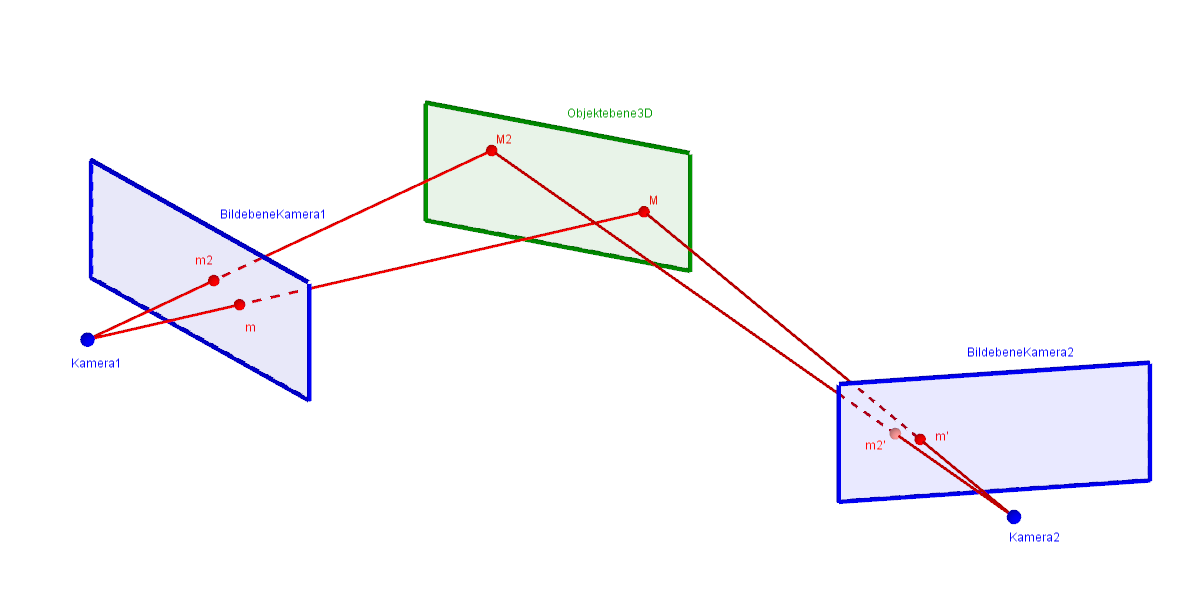
\includegraphics[width=1.\linewidth]{images/HomographieGrafik.png}
	\captionof{figure}{Veranschaulichung der Homographie bei zwei verschieden translatierten und rotierten Kameras. $(\vec{CO})$ und $(\vec{C'O})$ sind jeweils die Vektoren welche von den Abbildungspunkten $m$ beziehungsweise $m'$ ausgehen und sich im Objektpunkt $M$ treffen.}  
\end{minipage}\\ \\


Im folgenden wird das breits bekannte Beipiel für die Drehung um das Projektionszentrum, für die Drehung um einen Drehpunkt umgebaut. Danach soll nach dem gleichen Verfahren wie im vorherignen Beispiel aufgezeigt wurde eine Homographiematrix ermittelt werden, welche die Bildebenenkoordinaten der einen Kamera in die der anderen Kamera überführen kann. Die Herangehensweise für  dieses Beispiel größtenteils die selbe wie in dem Beispiel zuvor.Der unterschied liegt lediglich in der Transformation der Punkte in as Koordinatensystem von der gedrehten Kamera zwei. Diese besteht, im Gegensatzt zum vorherigen Beispiel, nicht nur aus hintereinander geschalteten Rotationen, sondern beinhlatet des Weiteren noch zwei Translationen. Die komplette Transformationsmatrix wird, um der vorherigen Notation gerecht zu bleiben, wieder mit $R$ beziehungsweise $R'$ notiert, auch wenn es sich hier nicht mehr um eine Reine Rotation handelt. In der Literatur wird die gesamte Transformationsmatrix ebenfalls mit $R$ notiert\cite{HZ,Elements,Schwarz}. $R$ und $R'$ bestehen aus insgesamt drei Transformationsmatrizen \ensuremath{R = \text{Verschiebung}_1 \cdot \text{Rotation} \cdot \text{Verschiebung}_2}. Da die Position des Projektionszentrums von Kamera zwei nicht mehr mit dem von Kamera eins übereinstimmt, muss diese erst mit Hilfe einer Tranformationsmatrix $T$ berechnet werden. $C_{\delta} = [0 \;0 \;0\; 1]$ sind die Koordinaten von Kamera eins in Weltkoordinaten. Da in diesem Beispiel das Kamerakoodrinatensystem von Kamera eins und das Weltkoordinatensystem deckungsgleich sind heißt das,  $C_{\beta} = [0 \;0 \;0\; 1]$. somit ist Matrix $R$, welche die Transformation der ersten Kamera im Bezug auf das Weltkoordinatensystem beschreibt gleich der Einheitsmatrix.

\begin{minipage}{\linewidth}
	\centering
	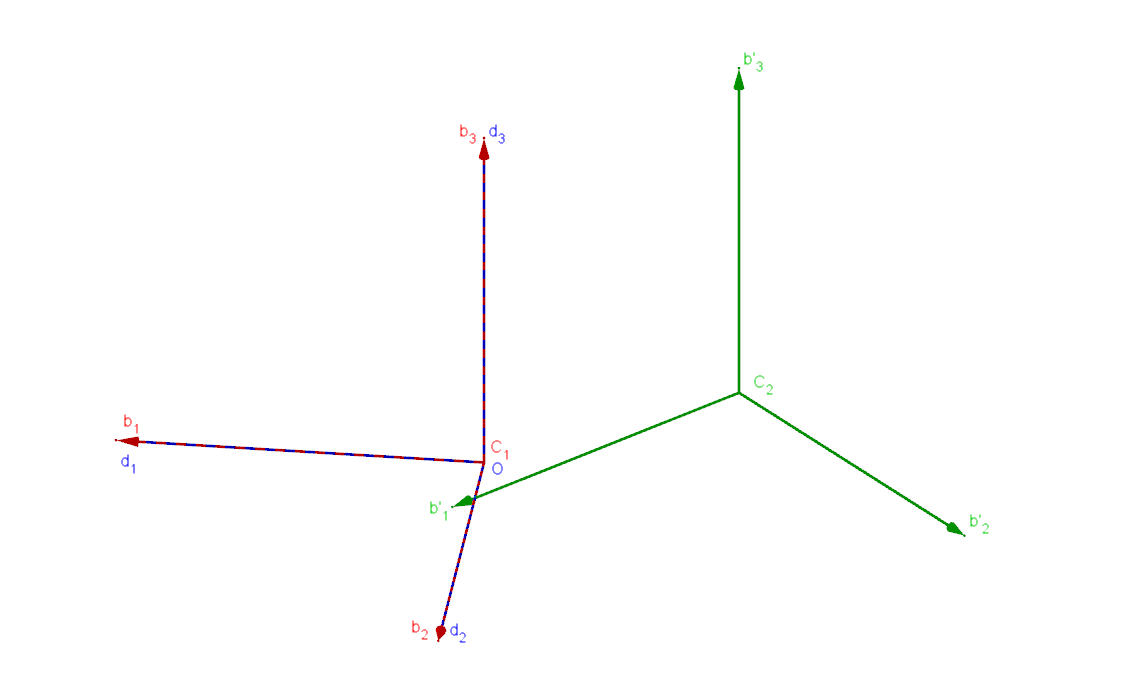
\includegraphics[width=1.\linewidth]{images/GrafikHomographieDifferentC.png}
	\captionof{figure}{Weltkoordinatensystem $(O,\delta)$ mit $\delta = [\vec{d_1},\vec{d_1},\vec{d_1},O]$ und Kamerakoordinatensysteme $\beta= [\vec{b_1},\vec{b_2},\vec{b_3},C]$ und $(C',\beta')$ mit $\beta'= [\vec{b'_1},\vec{b'_2},\vec{b'_3},C']$ .}
\end{minipage}\\ \\

Mit $C'$ wird der Ursprung des Koordinatensystems von Kamera zwei bezeichnet. Als Objekte in der Ebene im $\mathbb{R}^3$-Raum, werden die selben Punkt $A_\delta,B_\delta,C_\delta,D_\delta$ und $E_\delta$ wie im vorherigen Beispiel verwendet.\\

\begin{gather}
A_\delta=\begin{pmatrix}
0\\0\\2\\1
\end{pmatrix}, 
B_\delta=
\begin{pmatrix}
1\\0\\2\\1
\end{pmatrix},
C_\delta=
\begin{pmatrix}
1\\1\\2\\1
\end{pmatrix},
D_\delta=
\begin{pmatrix}
0\\1\\2\\1
\end{pmatrix},
E_\delta=
\begin{pmatrix}
\frac{1}{2}\\\frac{1}{2}\\2\\1
\end{pmatrix}
\end{gather}\\

Punkt $E_\delta$ bildet den Mittelpunkt des Quadrates und wird als Drehpunkt gewählt und mit $\textit{PivotPoint}$ bezeichnet. Als nächstes wird Matrix $T$ aus drei Transformationsmatrizen zusammengestellt. Diese Matrix verschiebt das Projektionszentrum von $C'$ an den gewünschten Ort im Weltkoordinatensystem. Bezeichnet werden die drei Matrizen mit $T_1, T_2$ und $T_3$. $T_1$ beinhaltet die Verschiebung von des Ursprungs von Kamera eins zum $\textit{PivotPoint}$, $T_2$ bildet die Rotationsmatrize, welche den Verschobenen Punkt um die gewünschten $45^\circ$ dreht. Die letzte Matrize $T_3$ beinhaltet wieder eine Translation, welche den Punkt vom $\textit{PivotPoint}$ zurück verschiebt. 

\begin{gather}
	T_1 = \begin{bmatrix}
	1&0&0&-\textit{PivotPoint}_x\\
	0&1&0&-\textit{PivotPoint}_y\\
	0&0&1&-\textit{PivotPoint}_z\\
	0&0&0&1
	\end{bmatrix} = 
	\begin{bmatrix}
	1&0&0&-\frac{1}{2}\\
	0&1&0&-\frac{1}{2}\\
	0&0&1&-2\\
	0&0&0&1
	\end{bmatrix}\\
	T_2 = \begin{bmatrix}
	\cos(45^\circ)&0&\sin(45^\circ)&0\\
	0&1&0&0\\
	-\sin(45^\circ)&0&\cos(45^\circ)&0\\
	0&0&0&1
	\end{bmatrix}=
	\begin{bmatrix}
	\frac{1}{\sqrt{2}}&0&\frac{1}{\sqrt{2}}&0\\
	0&1&0&0\\
	-\frac{1}{\sqrt{2}}&0&\frac{1}{\sqrt{2}}&0\\
	0&0&0&1
	\end{bmatrix}\\
	T_3 = 
	\begin{bmatrix}
	1&0&0&\textit{PivotPoint}_x\\
	0&1&0&\textit{PivotPoint}_y\\
	0&0&1&\textit{PivotPoint}_z\\
	0&0&0&1
	\end{bmatrix} = 
	\begin{bmatrix}
	1&0&0&\frac{1}{2}\\
	0&1&0&\frac{1}{2}\\
	0&0&1&2\\
	0&0&0&1
	\end{bmatrix}\\
	T= 
	T_3 \cdot T_2 \cdot T_1
	= 
	\begin{bmatrix}
	\frac{1}{\sqrt{2}}&0&\frac{1}{\sqrt{2}}&-1.26777\\
	0&1&0&0\\
	-\frac{1}{\sqrt{2}}&0&\frac{1}{\sqrt{2}}&0.93934\\
	0&0&0&1
	\end{bmatrix}\\
	C'_\delta = T \cdot C_\delta
	 = 	
	 \begin{bmatrix}
	\frac{1}{\sqrt{2}}&0&\frac{1}{\sqrt{2}}&-1.26777\\
	0&1&0&0\\
	-\frac{1}{\sqrt{2}}&0&\frac{1}{\sqrt{2}}&0.93934\\
	0&0&0&1
	\end{bmatrix} \cdot 
	\begin{bmatrix}
	0\\0\\0\\1
	\end{bmatrix}
	=
	\begin{bmatrix}
	-1.27\\0\\0.94\\1
	\end{bmatrix}	
\end{gather} 

Der Ursprung des Koordinatensystems von Kamera zwei befindet sich, angegeben in Weltkoordinaten, bei $C'_\delta =\begin{bmatrix}-1.26777&0&0.93934&1\end{bmatrix}^T$. Da nun die $C'_\delta$ bekannt ist, können die 3D-Objektpunkte in das Kamerakoordinatensystem von Kamera zwei transformiert werden. Hierzu wird die Matrix $R'$ aufgestellt.

\begin{gather}
	R' = \begin{bmatrix}
	&&&\\
	&[T_2]^{-1}&& -[T_2]^{-1} \cdot V\\
	&&&\\
	0&0&0&1\\
	\end{bmatrix}
\end{gather}

aufgestellt werden. $V$ ist der Translationsvektor welcher den Wert von $C'_\delta$ bekommt. Da es sich wieder um kartesische Koordinatensysteme handelt gilt wieder $[T_2]^{-1}$ = $[T_2]^{T}$.

\begin{gather}
	 -[T_2]^{T}\cdot C'_\delta = 
	 \begin{pmatrix}
	 \frac{1}{\sqrt{2}}&0&-\frac{1}{\sqrt{2}}\\
	 0&1&0\\
	 \frac{1}{\sqrt{2}}&0&\frac{1}{\sqrt{2}}
	 \end{pmatrix}
	 \cdot
	 \begin{pmatrix}
	 -1.27\\0\\0.94
	 \end{pmatrix}
	 =
	  \begin{pmatrix}
	 1.56\\0\\0.23
	 \end{pmatrix}
\end{gather}

Für die Transformationsmatrizen $R$ und $R'$ gilt dann jeweils:

\begin{gather}
	R = 
	\begin{bmatrix}
	1&0&0&0\\
	0&1&0&0\\
	0&0&1&0\\
	0&0&0&1
	\end{bmatrix}\\	
	R'=
	 \begin{bmatrix}
	\frac{1}{\sqrt{2}}&0&-\frac{1}{\sqrt{2}}&1.56\\
	0&1&0&0\\
	\frac{1}{\sqrt{2}}&0&\frac{1}{\sqrt{2}}&0.23\\
	0&0&0&1
	\end{bmatrix}
\end{gather}\\

Nachdem $R$ und $R'$ bestimmt sind,  müssen die Punkte in Weltkoordinaten noch in die entsprechenden Kamerakoordinatensysteme und mit den Projektionsmatrizen $K$ und $K'$ in deren Bildkoordinatensysteme transformiert werden. Es gilt wieder wie im Beispiel zuvor, dass $K = K'$ ist.

 \begin{gather}
 \leftidx{_{K_{c1}}}{\begin{bmatrix}
 	\pi
 	\end{bmatrix}}{_{K_{c1}}}
 =		\leftidx{_{K_{c2}}}{\begin{bmatrix}
 	\pi
 	\end{bmatrix}}{_{K_{c2}}}
 =
 \begin{pmatrix}
 \zeta&0&0&0\\
 0&\zeta&0&0\\
 0&0&\zeta&0\\
 0&0&1&0
 \end{pmatrix}=
 \begin{pmatrix}
 -1&0&0&0\\
 0&-1&0&0\\
 0&0&-1&0\\
 0&0&1&0
 \end{pmatrix}
 \end{gather}
 
 Es entstehen die folgenden beiden Punktematrizen $pC$ für Kamera eins und $pC'$ für Kamera zwei. Die Koordinaten der jeweiligen Punkte $ pC = [A_\tau \;B_\tau\;C_\tau\;D_\tau\;E_\tau$] und $pC' =[A_{\tau'}\;B_{\tau'}\;C_{\tau'}\;D_{\tau'}\;E_{\tau'}]$ aus Sicht der beiden Kameras befinden sich der Reihe nach in den Spalten der Punktematrix.
 
 \begin{gather}
 	pC = 
 	\begin{bmatrix}
 	0&\frac{1}{2}&\frac{1}{2}&0&\frac{1}{4}\\
 	0&0&\frac{1}{2}&\frac{1}{2}&\frac{1}{4}\\
 	1&1&1&1&1
 	\end{bmatrix}\\
 	pC'=
 		\begin{bmatrix}
 	0.09&0.36&0.36&0.09&\frac{1}{4}\\
 	0&0&0.42&0.61&\frac{1}{4}\\
 	1&1&1&1&1
 	\end{bmatrix}\\
 \end{gather}

Die Homographiematrix wird durch aufstellen der Koeffizientenmatrix und anschließendes Bestimmen von $H \cdot x = 0$ oder durch findes desjenigen Vektors $\vec{x}$ für den $||H\cdot x||$ minimal wird. Da es sich auch hier nicht um einen überbestimmten Fall handelt, kann die homographiematrix entweder durch die Bestimmung des Kerns oder durch anwenden der Singulärwertszerlegung $SVD$, gewonnen werden. Die resultierende Homographiematrix sieht folgendermaßen aus.

\begin{gather}
	H = \begin{bmatrix}
	0.43&0&0.43\\
	0&0.6&0\\
	0.4&0&0.5
	\end{bmatrix}
\end{gather}

Wird $H$ auf die Punkte $pC$ angewandt, so liefert das Ergebnis die Punkte von $pC'$ und wird die Inverse $H^{-^1}$ auf die Punkte $pC'$ angewandt, so erhält man die Punkte von $pC$. Somit wurde bewiesen, dass Homographiematrizen immer zur Transformation von Punkte genutzt werden können, solange sich diese Punkte auf einer Ebene im Raum befinden. Die Definition der Homographie sagt aus, dass sowohl Tranlationen und Rotationen in der Homographiematrix vorkommen dürfen \cite{Roser} \cite{Peiffer}. Die Drehung um einen Drehpunkt ist nicht weiter als die Hintereinaderschaltung verschiedener Tranformationsmarizen. Das wichtigste Kriterium welches erfüllt sein muss, damit Homographien angewendet werden können ist, dass die Abbildungen der Punkte in allen Kameras auf einer Ebene sich befinden müssen.\cite{Elements}.

In der Abbildung \ref{fig:DrehungDrehpunkt} ist ein grüner Punkt zu sehen welcher sich in Gegensatz zu den anderen Punkte nicht auf der selben Ebene befindet. Dieser Punkt lässt sich nicht mit der errechneten Homographiematrix ineinander überführen. Mit Hilfe von Homographien, können die Positionen und Orientierung der jeweiligen Kameras zueinander ermittelt werden, jedoch nur wenn sich die Szenepunkte auf einer Ebene befinden. Ein Beispiel hierfür wäre zum beispiel die Aufnahme einer Gebäudefassade aus unterschiedlichen Kamerawinkeln und Positionen\cite{Elements}. Für eine Szenenrekonstruktion einer kompletten 3D-Szene reichen pure Homographien nicht aus, hierfür muss sich der geometrischen Eigenschaften der Epipolargeometrie bedient werden. 



%\section{Punkte in unterschiedlichen Ebenen}
%
%The perspective
%projection of a point X by a camera with projection center C can be obtained
%geometrically in 3D affine space by taking all lines passing through the points C and
%X and finding the intersections with the (affine) image plane $\pi$.
%Three different situations may arise, Figure 9.1.\\
%
%1. If X 
%C, then there is an infinite number of lines passing through C 
%X,
%which intersect  $\pi$ in all its points, and therefore the projection of X contains
%the whole plane  $\pi$.\\
%
%2. If point Y != C lies in the plane  $\sigma$, which is parallel to  $\pi$ and passing through
%C, then the line passing trough C and Y (which there is exactly one) does not
%intersect the projection plane  $\pi$, and therefore, the projection of X is empty.\\
%
%3. If X does not lie in the plane  $\sigma$, then there is exactly one line passing through
%points C and X and this line intersects the projection plane  $\pi$ in exactly one
%point x. Hence the projection of X contains exactly one point x.\\
%
%Graphik zur Homographie anfertigen um einen Verlgeich der Punktebeziehungen zwischen epipolargeometrie und Homographie zu veranschaulichen 
%
%
%Überleitung zur Epipolargeometry.\\
%Warum kann hier keine Homographie benötigt werden\\
%was muss hier genutzt werden?\\
%
%$H$ berücksichtigt nicht die Tiefe der Punkte. Für $H$ müssen alle Punkte in einer Ebene liegen, nur so kann die Korrekte $H$ und somit die Translation und Rotation der Kamera berechnet werden. Werden Punkte aus einer 3D-Szene auf ein 2D Bild gemapped, sollte man denken, dass mit Hilfe von $H$ die Punkte auf diesen Bildern ineinander überführt werden könnten. Dem ist jedoch nicht so, da die Punkte in unterschiedlichen Tiefen liegen, werden sie natürlich anders auf eine 2D-Ebene gemapped als wenn sie sich in der selben Tiefen befinden würden. Was benötigt wird ist also die sogenannte Epipolargeometrie. Allem voran die Beziehungen von korrespondierenden Punkten zweier Bilder ausgedrückt durch die Fundamentalmatrix und der essentiellen Matrix.


 
%\section{Epipolargeometrie als Grundlage der Stereokalibrierung und Szenenrekonstrunktion}

%
%Die Epipolargeometrie beschreibt eine intrinsische projektive Geometrie zwischen zwei Bildern\cite{HZ}. Sie dient insbesondere zur Korrespondenzanalyse von Punkten aus Bildern und zur Gewinnung von 3-D-Informationen. Ohne Kenntnis der Kamerapositionen, kann mit Hilfe der Epipolargeometrie eine einfache Beziehung zwischen korrespondierenden Punkten hergestellt werden. Abbildung 3.12 zeigt, den Aufbau zweier Kameras mit ihren Projektionszentren $C$ und $C'$, deren Bildebenen $I$ und $I'$, welche vor den Projektionszentren platziert wurden. Die Bildebenen können sich auch hinter den Projektionszentren befinden, das hat letztendlich keinen Einfluss auf die geometrischen Beziehungen\cite{HZ}. Zu den Elementen der Epipolargeometrie gehören zum einen die Epipole $e$ und $e'$. Betrachtet man die Basislinie zwischen den beiden Projektionszentren, so entsteht der Epipol genau am Schnittpunkt der Verbindungslinie mit den jeweiligen Bildebenen. Tritt der Fall ein, dass die Basislinie parallel zu einer oder beiden Bildebenen ist, so kommt es zu keiner Abbildung des Epipols auf den entsprechenden Bildebenen, sondern der Epipol befindet sich in diesem Falle im unendlichen\cite{ZZGXr}. Das hat zur Folge, dass alle Epipolarlinien, welche durch den Epipol verlaufen, sich zueinander parallel anordnen. Epipolarlinien die Linien, welche durch einen Bildpunkt $m$ oder $m'$ und dem jeweiligen Epipol $e$ oder $e'$ des Bildes verlaufen. Der Korrespondierende Punkt zu $m$ ist $m'$ und die korrespondierende Epipolarlinie $l'$ zu $m$, ist diejenige Linie, welche durch $m'$ und $e'$ verläuft. 
%
%
%\begin{minipage}{\linewidth}
%	\centering
%	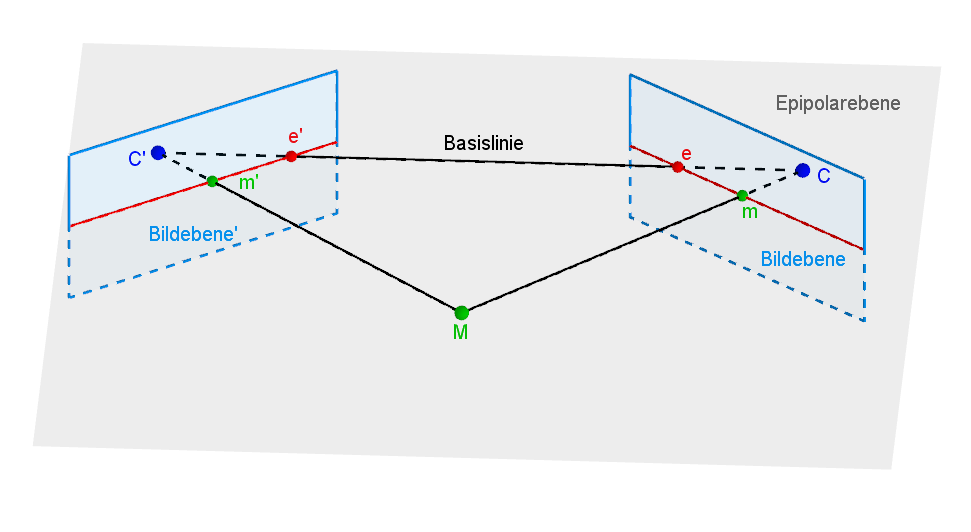
\includegraphics[width=1.\linewidth]{images/EpipolarGeoemtrieGrafik.png}
%	\captionof{figure}{Grafik zu den geometrischen Eigenschaften der Epipolargeometrie zwischen zweik Bildern. $C$ und $C'$ sind die Projektionszentren zweier Kameras. Beide Kameras besitzen jeweils eine Bildebene. Die Basislinien verbindet die Projektionszentren der Kameras. Der Punkt an welchem die Basislinie die Bildebenen schneidet, wird als Epipol bezeichnet. Durch den Epipol verlaufen alle Epipolarlinien des Bildes. $M$ ist der Objektpunkt im 3D-Raum und $m_1$ und $m_2$ sind die jeweiligen Abbildungen dieses Punktes auf den Bildebenen. Die Verbindungsvektoren zwischen $C, C'$ und $M$ bilden die sogenannte Epipolarebene\cite{Elements,HZ,ZZGXr}.}  
%\end{minipage}\\ \\
%
%
%Die Epipolarlinie $l'$, beinhaltet alle möglichen korrespondierenden Punkte zu $m$. Wenn $C$ auf seiner Bildebene $I$ einen Punkt $m$ abbildet, so erscheint dieser Punkt immer an der selben Stelle auf dem 2D - Bild, egal wie nah der Ursprüngliche 3D-Objektpunkt $M$ an $I$ befindet. Rein theoretisch, könnte der Originial Szenenpunkt $M$, sich überall auf der Verbindungslinie $\bar{Mm}$ befinden. Der Abgebildete Punkt $m$ wäre auf $I$ immer an der selben Stelle abgebildet. Fährt man nun mit $M$ die Verbindungslinie $\bar{Mm}$ entlang, dann ist $m$ immer an der selben Stelle auf $I$ zu sehen, während der korrespondierende Punkt $m'$ sich entlang der Epipolarlinie bewegen würde. Die Epipolargeometrie beschreibt also eine Beziehung zwischen einem Bildpunkt $m$ und dessen korrespondierender Epiplolarlinie $l'$, welche wiederum alle möglichen zu $m$ korrespondierenden Punkte $m'$ beinhaltet\cite{HZ,Zhang2014,ZZGXr}.\\
%
%
%
%\begin{minipage}{\linewidth}
%	\centering
%	\includegraphics[width=1.\linewidth]{images/EpipolarLinien.png}
%	\captionof{figure}{Die Objektpunkte $M_1, M_2$ und $M_3$ werden in $I'$ als $m'_1, m'_2$ und $m'_3$ abgebildet, während sie in $I$ immer den selben Bildpunkt $m_1$ ergeben.}  
%\end{minipage}\\ \\
%
%
%Die Epipolargeometrie lässt sich, ähnlich wie eines Homographiematrix, in einer 3x3-Matrix zusammenfassen. Diese ist jedoch singulär und besitzt somit nicht wie die Homographiematrix Rang 3 sondern Rang 2. Je nachdem ob ein ein kalibriertes oder unkalibriertes System vorliegen hat, handelt es sich entweder um die sogenannten Fundamental Matrix $F$ oder die Essentielle Matrix $E$ \cite{Elements,HZ,ZZPaper,Zhang2014,ZZGXr}. Von der Fundamentalmatrix $F$ ist dann die rede, wenn die intrinsischen Kameraparameter nicht bekannt sind, sprich wenn das System unkalibriert ist. In diesem Fall wird mit Bildpixelkoordinaten gearbeitet. Sind die intrinsischen Parameter bekannt, so wir $F$ zur essentiellen Matrix $E$ und es wird mit sogenannten normalisierten Bildkoordinaten gearbeitet\cite{ZZPaper}. Was genau die unterschiedlichen Koordinaten ausmacht, wird in Kapitel (KAPITELLINK) genauer erklärt. Mathematisch sagen die Matrizen $F$ und $E$ in Verbindung mit den korrespondierenden Punkten aus, ob für einen Bildpunkt $m$ in einer Kamera, dessen korrespondierender Bildpunkt $m'$ in der anderen Kamera auf der korrespondierenden Epipolarlinie liegt.  Das heißt, wenn $m'Fm = 0$ oder $\hat{m'}E\hat{m}= 0$, dann ist der sogenannte \textit{epipolar-constraint} erfüllt. Der \textit{epipolar-constraint} gibt somit Aufschluss darüber, ob $m'$ ein möglicher korrespondierender Punkt von $m$ ist. Dies ist nämlich genau dann der Fall, wenn $m'Fm = 0$ oder $\hat{m'}E\hat{m}= 0$ sind\cite{HZ,Zhang2014}. Ist der \textit{epipolar-constraint} erfüllt, so wird gleichzeitig der Suchaufwand nach weiteren Korrespondenzen reduziert, da somit nur noch eine eindimensionale Suche, entlang der Epipolarlinie, anstatt einer zweidimensionalen durchgeführt werden muss. Dieser neue \textit{contraint} wird auch als \textit{coplanarity constraint} oder Koplanaritätsbeschränkung bezeichnet. Dieser entsteht, da die Projektionszentren der Kameras und die korrespondierenden Bildpunkte auf ein und der selben Ebene liegen müssen \cite{Zhang2014}. Die Epipolargeometrie und die in ihr beinhalteten $constraints$, helfen bei der 3D-Szenenrekonstruktion. Szenenrekonstruktion ist dann möglich, wenn in einer Stereoaufnahme in beiden Bildern die zueinander gehörenden Bildpunkte lokalisiert wurden. Wird also eine Szene mit zwei Kameras aufgenommen, so liegen während der Aufnahme die aufgenommenen Objekpunkte, das Projektionszentrum und der zur Kamera gehörende Bildpunkt auf einer Linie. Wurde eine Objektpunkt nun zweimal aus verschiedenen Winkeln und/ oder Position aufgenommen, lassen sich nachdem die extrinsischen Parameter der Kameras ermittelt wurden, die Schnittpunkt der jeweiligen Linien aus Kamera eins und Kamera zwei berechnen. Diese Schnittpunkte ergeben den ursprünglichen Objektpunkt. Die Szene ist somit rekonstruiert\cite{Elements,ZZGXr,HZ}. 
%
%
%\section{Geometrische Erläuterung der Fundamentalmatrix und der Essentiellen Matrix }
%
%Nachdem die Theorie der geometrischen Hintergründe der Epipolargeometrie, bei der Stereokalibrierung und Szenerekonstruktion, erläutert wurden, wird nun der mathematische Hintergrund genauer aufgezeigt. Vor allem soll auf die Herleitung der neu eingeführten Fundamental Matrix $F$ und der essentiellen Matrix $E$ eingegangen werden. Diese spielen nämlich eine entscheidende Rolle bei der Rekonstruktion der Kamerapose und der Szenenrekonstruktion\cite{Elements, HZ}. $F$ und $E$ bilden jeweils eine singuläre 3x3-Matrix, welche die Geometrie zwischen den Bildpunkten $m_\tau$ und $m'_\tau$ auf $I$ und $I'$ und dem Objektpunkt $M_\delta$ im Raum beschreibt. Die Vektoren $\overline{CM} = (\vec{M}_\delta - \vec{C}_\delta),\, \overline{C'M} = (\vec{M}_\delta - \vec{C'}_\delta)$ und $\overline{CC'} = (\vec{C'}_\delta - \vec{C}_\delta)$ bilden das in Abbildung 3.12 sichtbare schwarze Dreieck. $F$ und $E$ fassen dieses Dreieck in ihren Matrizen zusammen. Um das ganze mathematisch zu erklären, wird ein Stereokameraufbau definiert. Ein Objektpunkt $M_\delta$ in Weltkoordinaten$(O,\delta)$ wird von zwei Kameras $C$ mit $(C,\beta)$ und $C'$ mit $(C',\beta')$ aufgenommen und auf deren Bildebenen $I$ und $I'$ als $m_\beta$ und $m'_\beta$ abgebildet. $C$ und $C'$ besitzen jeweils eine eigene Projektionsmatrix $P$ und $P'$. Anzumerken ist, dass die folgende Herleitung nach \cite{Elements} aufgestellt wurde.
%
%\begin{gather}
%	P = \begin{bmatrix}
%	KR|-KR\vec{C}_\delta
%	\end{bmatrix}\\
%	P' = \begin{bmatrix}
%	K'R'|-K'R'\vec{C'}_\delta
%	\end{bmatrix}
%\end{gather}
%
%$M$ wird mit $P$ und $P'$ auf die Bildebenen $I$ und $I'$ mit den jeweiligen Koordinatensystemen $I = (I,\tau)$ und $I'= (I',\tau')$ projiziert. Wichtig anzumerken, auch für den späteren Aufbau mit zwei Kameras unterschiedlicher Auflösung, ist, dass es sich bei den Koordinatensystemen von $I$ und $I'$ nicht um identische handeln muss.\cite{Elements} Es entstehen die Bildpunkte $\gamma m_\tau$ und $\gamma' m'_{\tau'}$ mit $\gamma \geq 0$ und $\gamma' \geq 0$. (gamma erklären)
%
%\begin{gather}
%	\gamma\vec{m}_\tau = P \begin{bmatrix}\vec{M}_\delta\\1\end{bmatrix}\\
%	\gamma\vec{m}_\tau = \begin{bmatrix}KR|-KR\vec{C}_\delta\end{bmatrix}\begin{bmatrix}\vec{M}_\delta\\1\end{bmatrix}\\
%	\gamma'\vec{m'}_{\tau'} = P' \begin{bmatrix}\vec{M}_\delta\\1\end{bmatrix}\\
%	\gamma'\vec{m'}_{\tau'} = \begin{bmatrix}K'R'|-K'R'\vec{C'}_\delta\end{bmatrix}\begin{bmatrix}\vec{M}_\delta\\1\end{bmatrix}\\
%\end{gather}
%
%$-KR\vec{C}_\delta$ und $-K'R'\vec{C'}_\delta$ verrechnet mit $M$ sind gleich den Vektorausdrücken $(\vec{M}_\delta - \vec{C}_\delta)$ und $(\vec{M}_\delta - \vec{C'}_\delta)$, welche die Verbindungslinie der beiden Projektionszentren mit dem Objektpunkt $M$ im Raum beschreiben.
%
%\begin{gather}
%	\gamma\vec{m}_\tau = KR(\vec{M}-\vec{C}_\delta)\\
%	\gamma'\vec{m'}_\tau = K'R'(\vec{M}-\vec{C'}_\delta)
%\end{gather}
%
%Gleichungen 3.89 und 3.90 werden nach $(\vec{M}-\vec{C}_\delta)$ und $(\vec{M}-\vec{C'}_\delta)$ aufgelöst.
%
%\begin{gather}
%	\gamma R^TK^{-1}\vec{m}_\tau = (\vec{M}-\vec{C}_\delta)\\
%	\gamma R'^TK'^{-1}\vec{m'}_{\tau'} = (\vec{M}-\vec{C'}_\delta)
%\end{gather}
%
%Wie bereits erwähnt ergibt sich aus den Vektoren $(\vec{M}_\delta - \vec{C}_\delta),\, (\vec{M}_\delta - \vec{C'}_\delta)$ und $(\vec{C'}_\delta - \vec{C}_\delta)$ das Dreieck aus Abbildung 3.12. Für das Dreieck kann, aus den drei Vektoren, die folgende Gleichung aufgestellt werden. 
%
%\begin{gather}
%	(\vec{C'}_\delta - \vec{C}_\delta) = (\vec{M}_\delta - \vec{C}_\delta) - (\vec{M}_\delta - \vec{C'}_\delta)
%\end{gather}
%
%$(\vec{M}-\vec{C}_\delta)$ und $(\vec{M} - \vec{C'}_\delta)$ können durch die Ausdrücke in den Gleichungen 3.91 und 3.92 ersetzt werden.
%
%\begin{gather}
%		(\vec{C'}_\delta - \vec{C}_\delta) = \gamma R^TK^{-1}\vec{m}_\tau - \gamma R'^TK'^{-1}\vec{m'}_{\tau'}
%\end{gather}
%
%Es gilt $\gamma \geq 0$ und $\gamma' \geq 0$, sie stehen für die Teife von $m$ und $m'$ und können mit Hilfe des Kreuzproduktes eliminiert werden\cite{Elements}. Zunächst wird $(\vec{C}'_\delta - \vec{C}_\delta)$ auf die rechte Seite gebracht, so dass die Gleichung nach Null aufgelöst wird.
%
%
%\begin{gather}
%	\begin{bmatrix}\vec{C'}_\delta - \vec{C}_\delta\end{bmatrix}_\times \gamma R^TK^{-1}\vec{m}_\tau - 
%	\begin{bmatrix}	\vec{C'}_\delta - \vec{C}_\delta\end{bmatrix}_\times \gamma' R'^TK'^{-1} \vec{m'}_{\tau'} =  0
%\end{gather}
%
%Gleichung 3.95 wird von links mit $\gamma' \vec{x'}^T_{\tau'}K'^{-T}R'$. Somit kann eine der beiden Schiefsymmetrischen Matrizen aus der Gleichung eliminiert werden. 
%
%\begin{gather}
%	\gamma' \vec{m'}_{\tau'} K'^{-T}R' \begin{bmatrix}	\vec{C'}_\delta - \vec{C}_\delta\end{bmatrix}_\times \gamma R^TK^{-1}\vec{m}_\tau = 0
%\end{gather}
%
%Da $\gamma \geq 0$ und $\gamma' \geq 0$, kann für Gleichung 3.96 auch folgendes geschrieben werden.
%
%\begin{gather}
%	 \vec{m'}_{\tau'} K'^{-T}R' \begin{bmatrix}	\vec{C'}_\delta - \vec{C}_\delta\end{bmatrix}_\times R^TK^{-1}\vec{m}_\tau = 0
%\end{gather}
%
%Aus Gleichung 3.97 können nun die Matrizen $F$ und $E$ ausgelesen werden. Bei $E$ handelt es sich um einen Kalibrierten Fall, dass bedeutet dass sowohl $K$ als auch $K'$ bekannt sind und die normalisierten Bildkoordinaten $\vec{\hat{m}}$ und $\vec{\hat{m}}'$  durch multiplikation mit $K$ und $K'$ entstehen. $E$ selbst fässt die Schiefsymmetrische Matrix $[\vec{C'}_\delta - \vec{C}_\delta]_\times$ und die beiden Transformationsmatrizen $R$ und $R'$ zusammen. 
%
%\begin{gather}
%	\vec{m'}_{\tau'}^T K'^{-T}EK^{-1}\vec{m}_\tau = 0\\
%	\vec{\hat{m}}_\tau^T E \vec{\hat{m}}'_{\tau'} = 0
%\end{gather}
%
%Matrix $E$ wird zu $F$, wenn es sich um einen unkalibrierten Fall handelt. Unkalibriert bedeutet, dass $K$ und $K'$ nicht bekannt sind, die Informationen zu $K$ und $K'$ in $F$ befinden. Werden $K$ und $K'$ zu $E'$ multipliziert, wird $E$ zu $F$. 
%
%\begin{gather}
%	\vec{m'}_{\tau'}^T K'^{-T}EK^{-1}\vec{m}_\tau = 0\\
%		\vec{m'}_{\tau'}^T F\vec{m}_\tau = 0
%\end{gather}
%
%$F$ und $E$, fassen die komplette Epipoloargeometrie, sprich externe und interne Parameter, sowie die geometrische Beziehung der jeweiligen Bildpunkte zu den 3-D Objektpunkten in einer 3x3-Matrix zusammen. Für $F$ und $E$ gibt es nicht nur eine Lösung. Werden $F$ oder $E$ Beispielsweise über den \textit{eight-Point-Algorithm} ermittelt, so sind die entstehenden 3x3-Matrixen und jedes vielfache von diesen gültige Lösungen für $F$ und $E$\cite{HZ,HZ8}. \textcolor{red}{Noch herausfinden ob das mit den Tiefen $\gamma$ und $\gamma'$ zusammenhängt!!}. Mit $F$ und $E$ kann wie bereits nachgeprüft werden, ob der \textit{epipolar-constraint} $m'^TFm = o$ oder $\hat{m'}^TE\hat{m} = 0$ zwischen zwei Bildpunkte gilt. Des weiteren können Epipole $e$ und $e'$ und Epipolarlinien $l$ und $l'$ ausfindig gemacht werden, sobald $E$ oder $F$ bekannt ist\cite{HZ,Elements,HZ8,ZZGXr}. Um die zu $m$ oder $m'$ korrespondierende Epipolarlinie $l'$ oder $l$ zu berechnen gilt:
%
%\begin{gather}
%l' = Fm\\
%l = F^Tm'
%\end{gather} 
%
%Um die Epipole $e$ und $e'$ zu berechnen die Gleichungen 3.103 und 3.104 erfüllt sein. Für $e$ reicht es also den rechten Nullraum von F zu bestimmen und für $e'$ muss dementsprechend der linke Nullraum von $F$ gefunden werden. 
%
%\begin{gather}
%	Fe = 0\\
%	F^Te' = 0
%\end{gather}
%
%Die Matrizen $F$ und $E$ sind die ausschlaggebenden Elemente, wenn es um die rekonstruktion der Kameraorientierungen und der Rekonstruktion der Szene geht. In beiden folgenden Kapitel werden zwei Beispiele zur Findung der exterenen Kameraparameter und der Szenenrekonstruktion aufgezeigt. Beim ersten Beispiel handelt es sich um ein Minimalbeispiel mit synthetisch erzeugten reinen Daten, um die theoretische Funktionalität des Algorithmus zu beweisen. Im zweiten Beispiel, wird der Algorithmus, mit einigen Anpassungen an die Realverhältnisse, auf Stereobildpaare, aufgenommen von zwei verschiedenen Kameras, angewandt. Die implementierten Algotithmen ermitteln aus einem Satz korrespondierender Bildpunkte die Fundamental Matrix und die essentielle Matrix mit Hilfe des sogenannten \textit{8-Point-Alhorithm}, Im Anschluss werden dann die externen Kameraparameter ermittelt und die Szene mit einem Triangulationsverfahren rekonstruiert. 
%
